\documentclass[12pt,a4paper,titlepage=true,parskip,ngerman]{scrartcl}
\usepackage[utf8]{inputenc}
\usepackage[T1]{fontenc}
\usepackage{lmodern}
\usepackage{microtype}
\usepackage{babel}
\usepackage{csquotes}
\usepackage{booktabs}
\usepackage{graphicx}
\usepackage{amsmath}
\usepackage{amssymb}
\usepackage{amsfonts}
\usepackage{mathtools}
\usepackage{bm}
\usepackage[table]{xcolor}
\usepackage{longtable}
\usepackage{colortbl}
\usepackage{rotating}
\usepackage{multicol}
\usepackage{multirow}
\usepackage{enumerate}
\usepackage{enumitem}


\begin{document}
%Thesen:\\
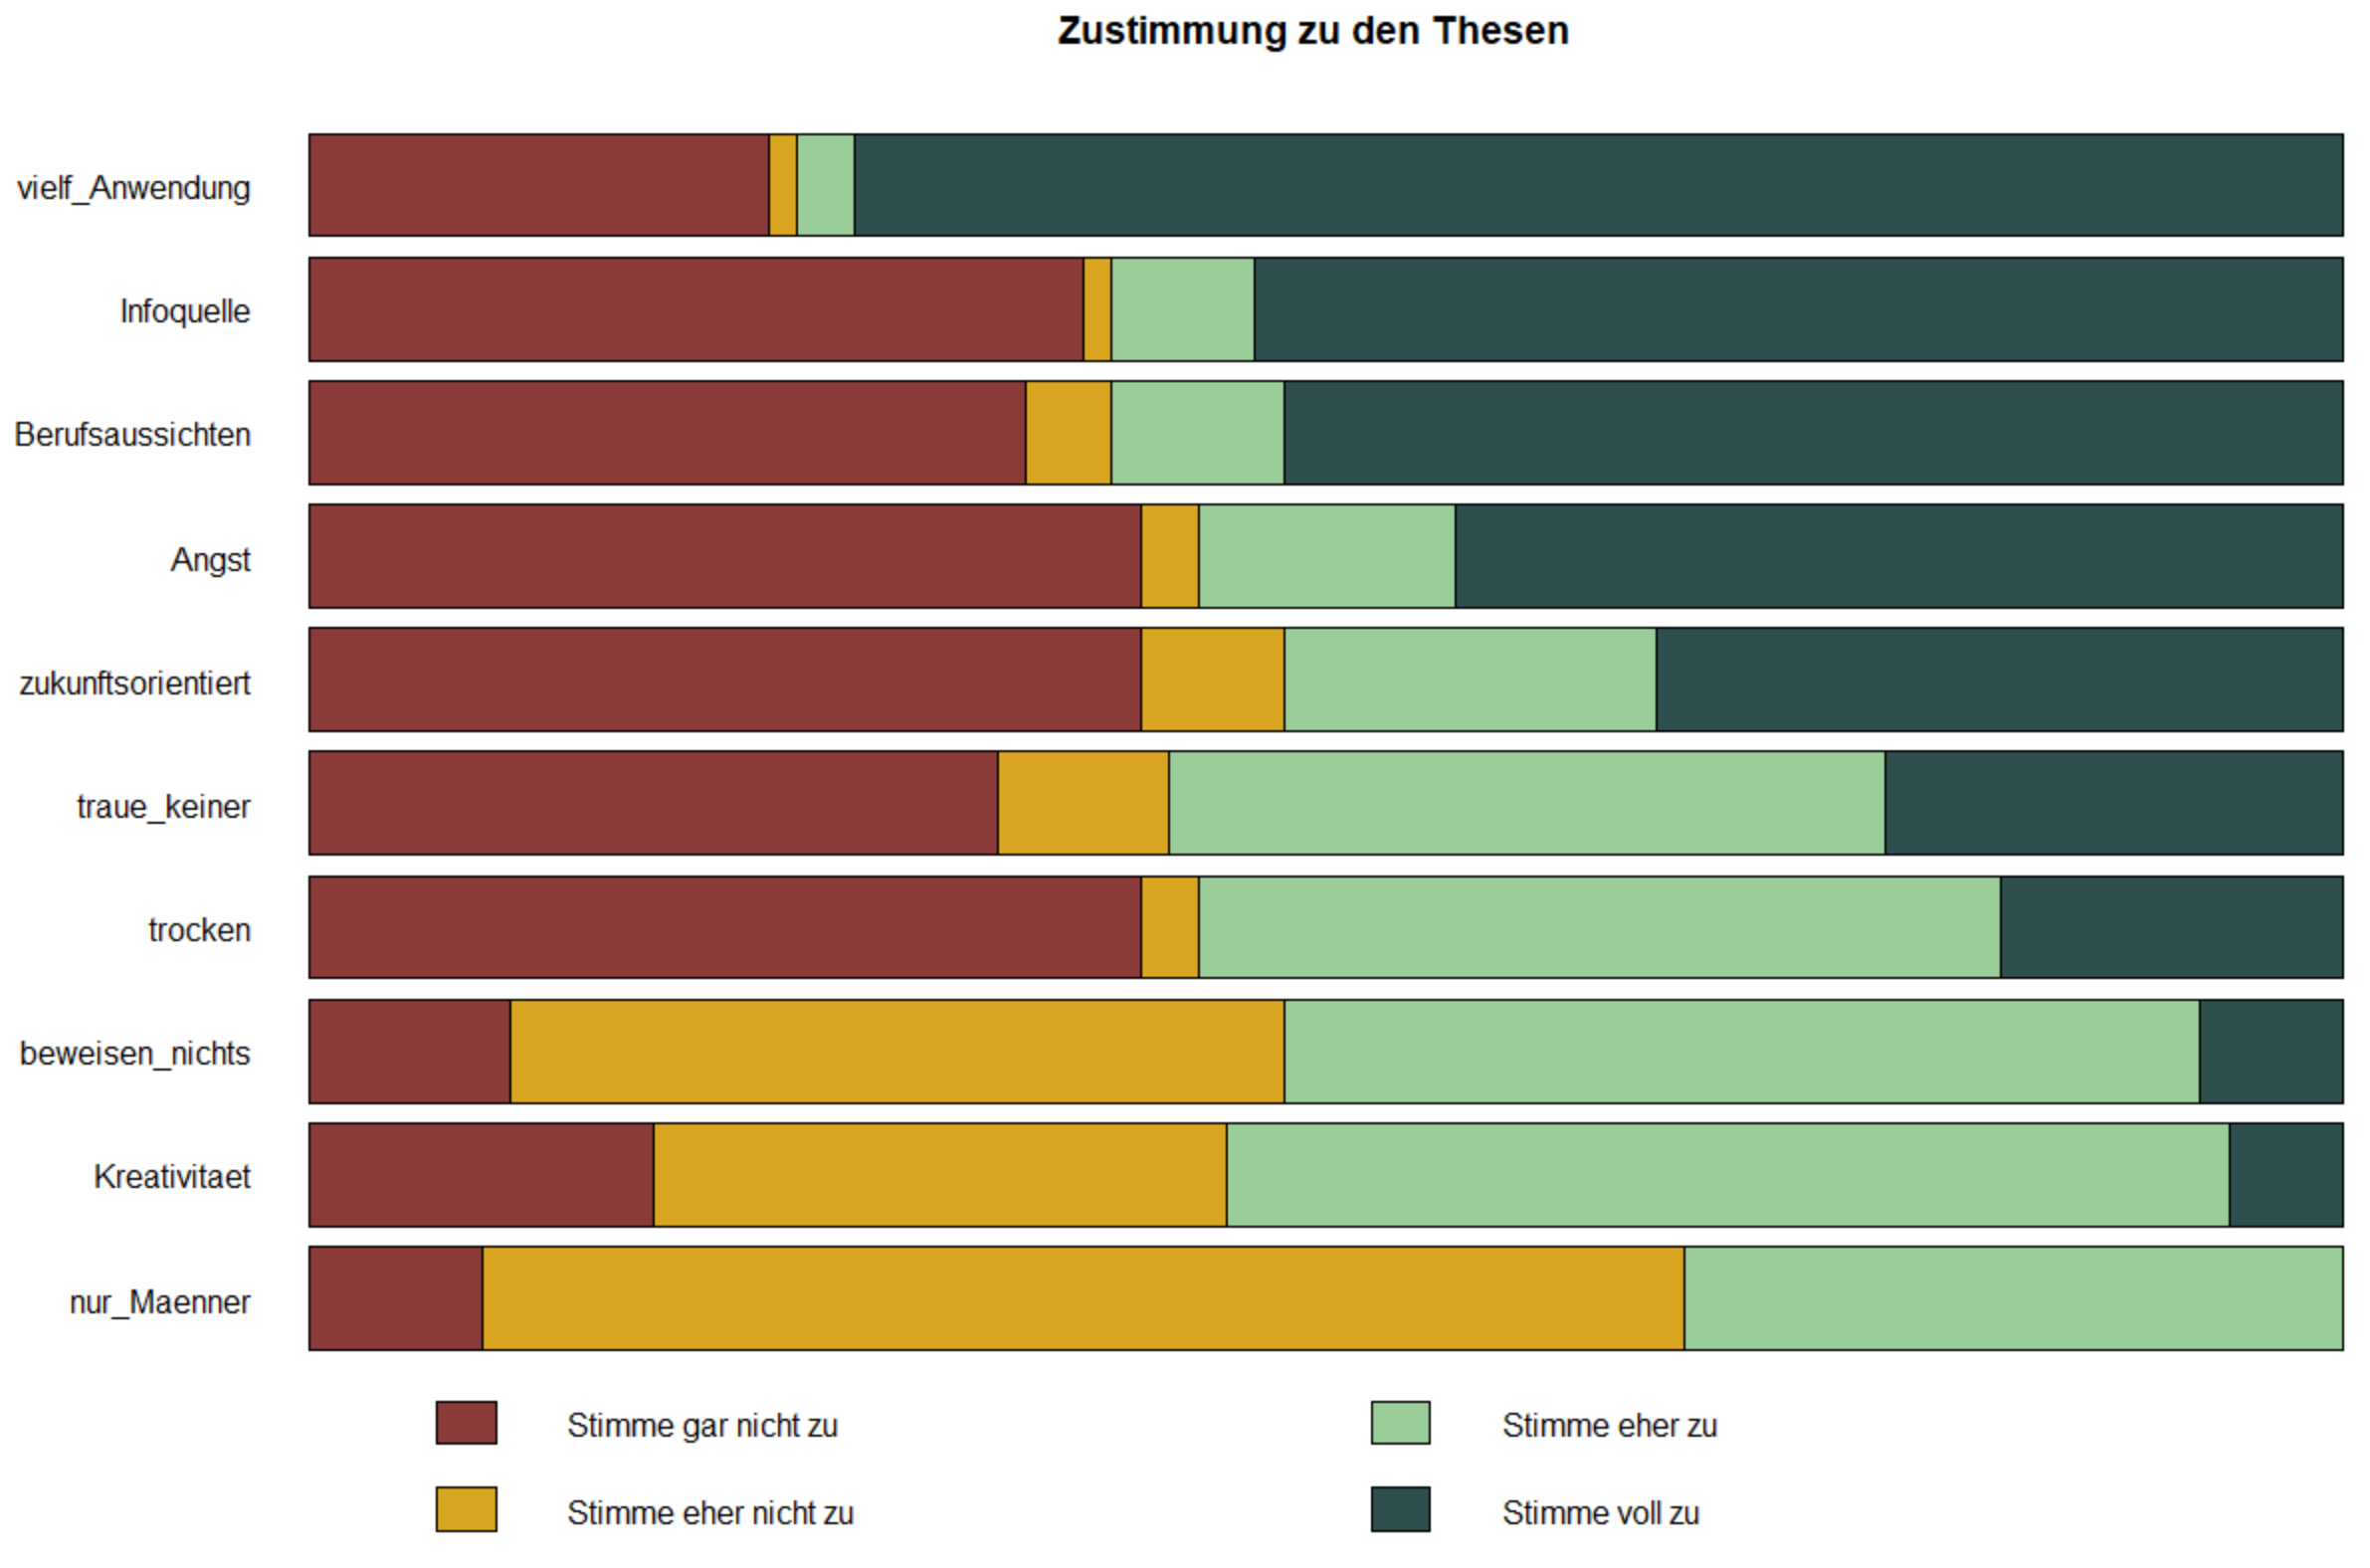
\includegraphics[scale=0.48]{gestapelter_Barplot_Thesen}
\vspace{0.2cm}

%Eigenschaften:
%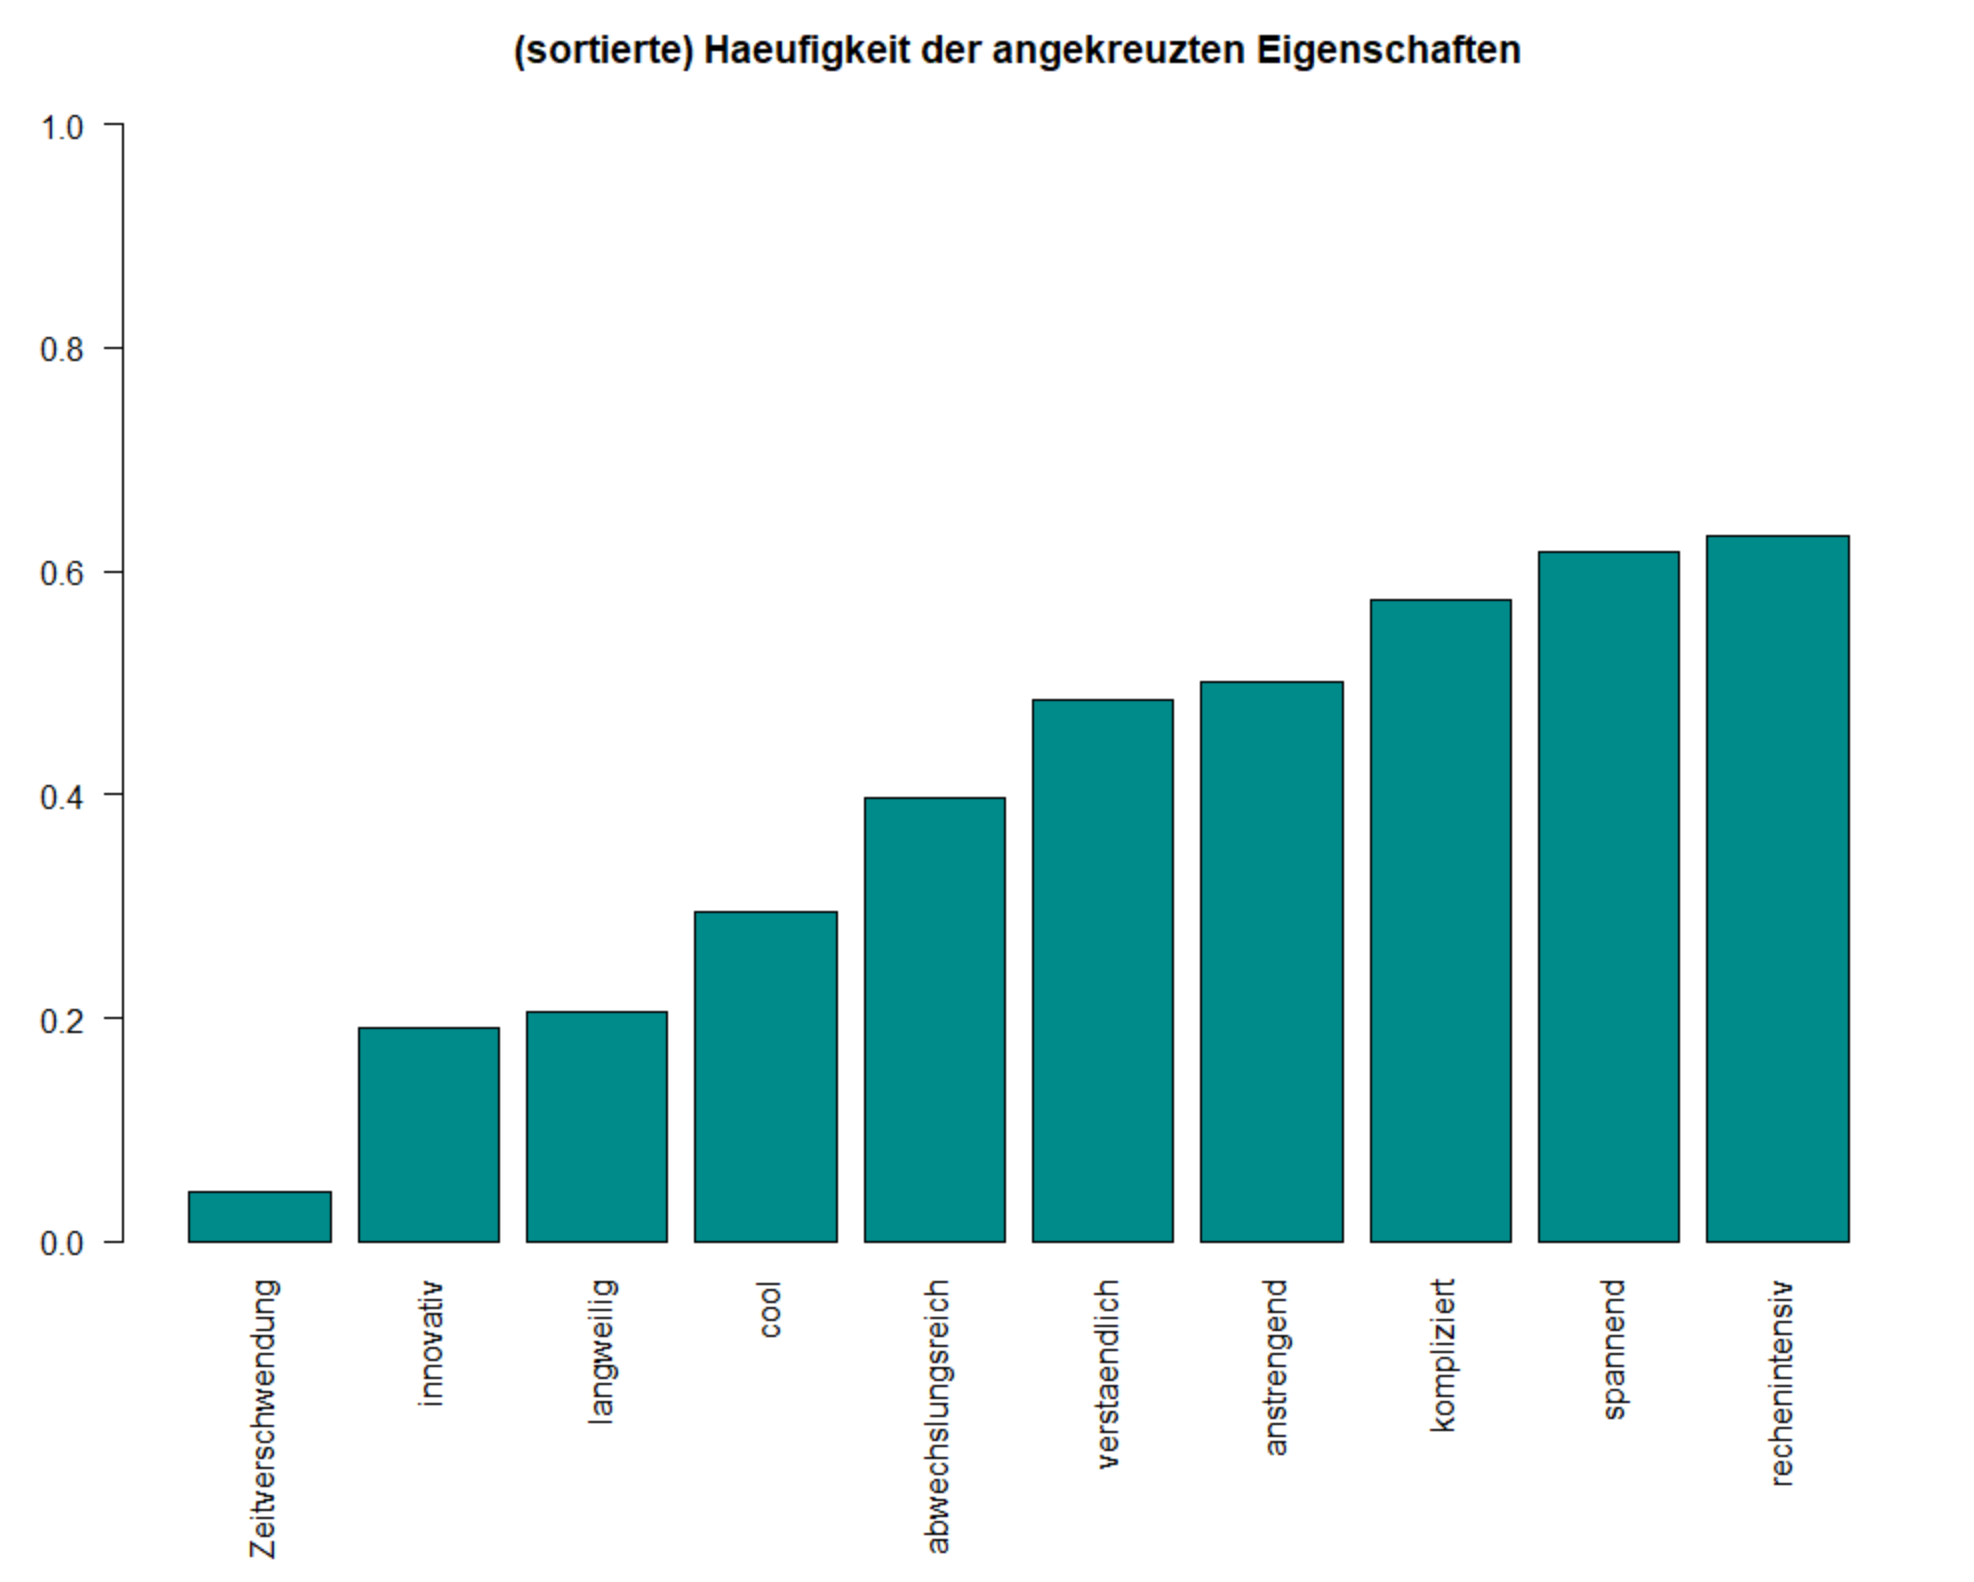
\includegraphics[scale=0.5]{sort_Hfgkeit_angekreuzter_Eigenschaften}
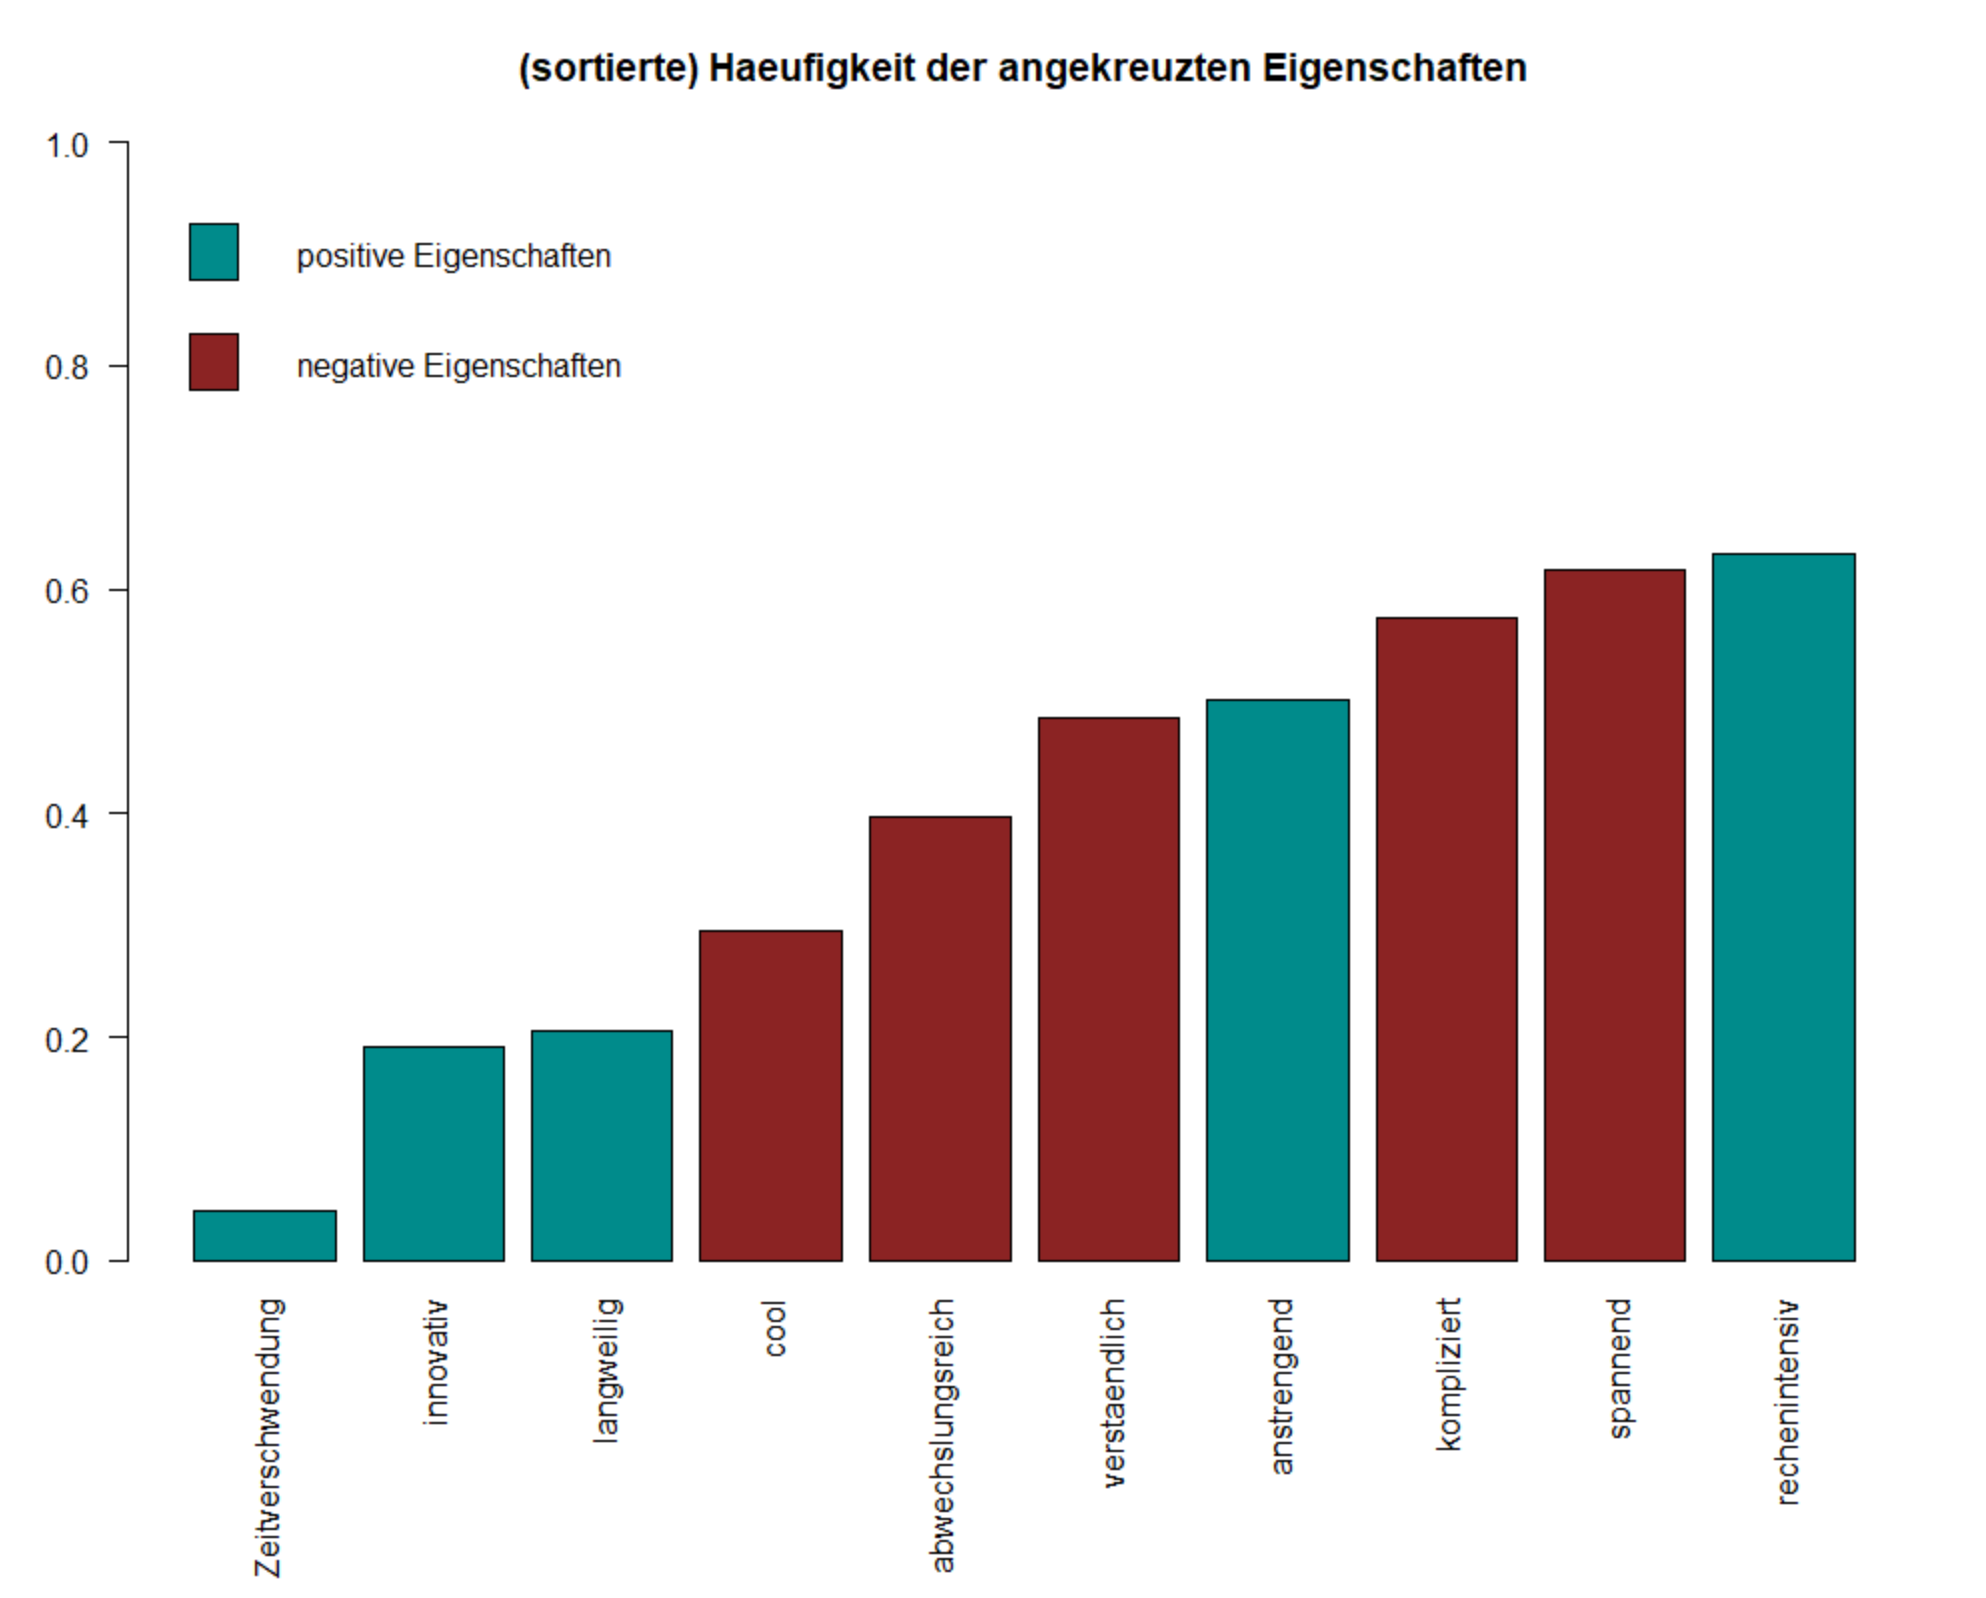
\includegraphics[scale=0.48]{sort_pos_neg_Hfgkeit_angekreuzter_Eigenschaften}\\	
%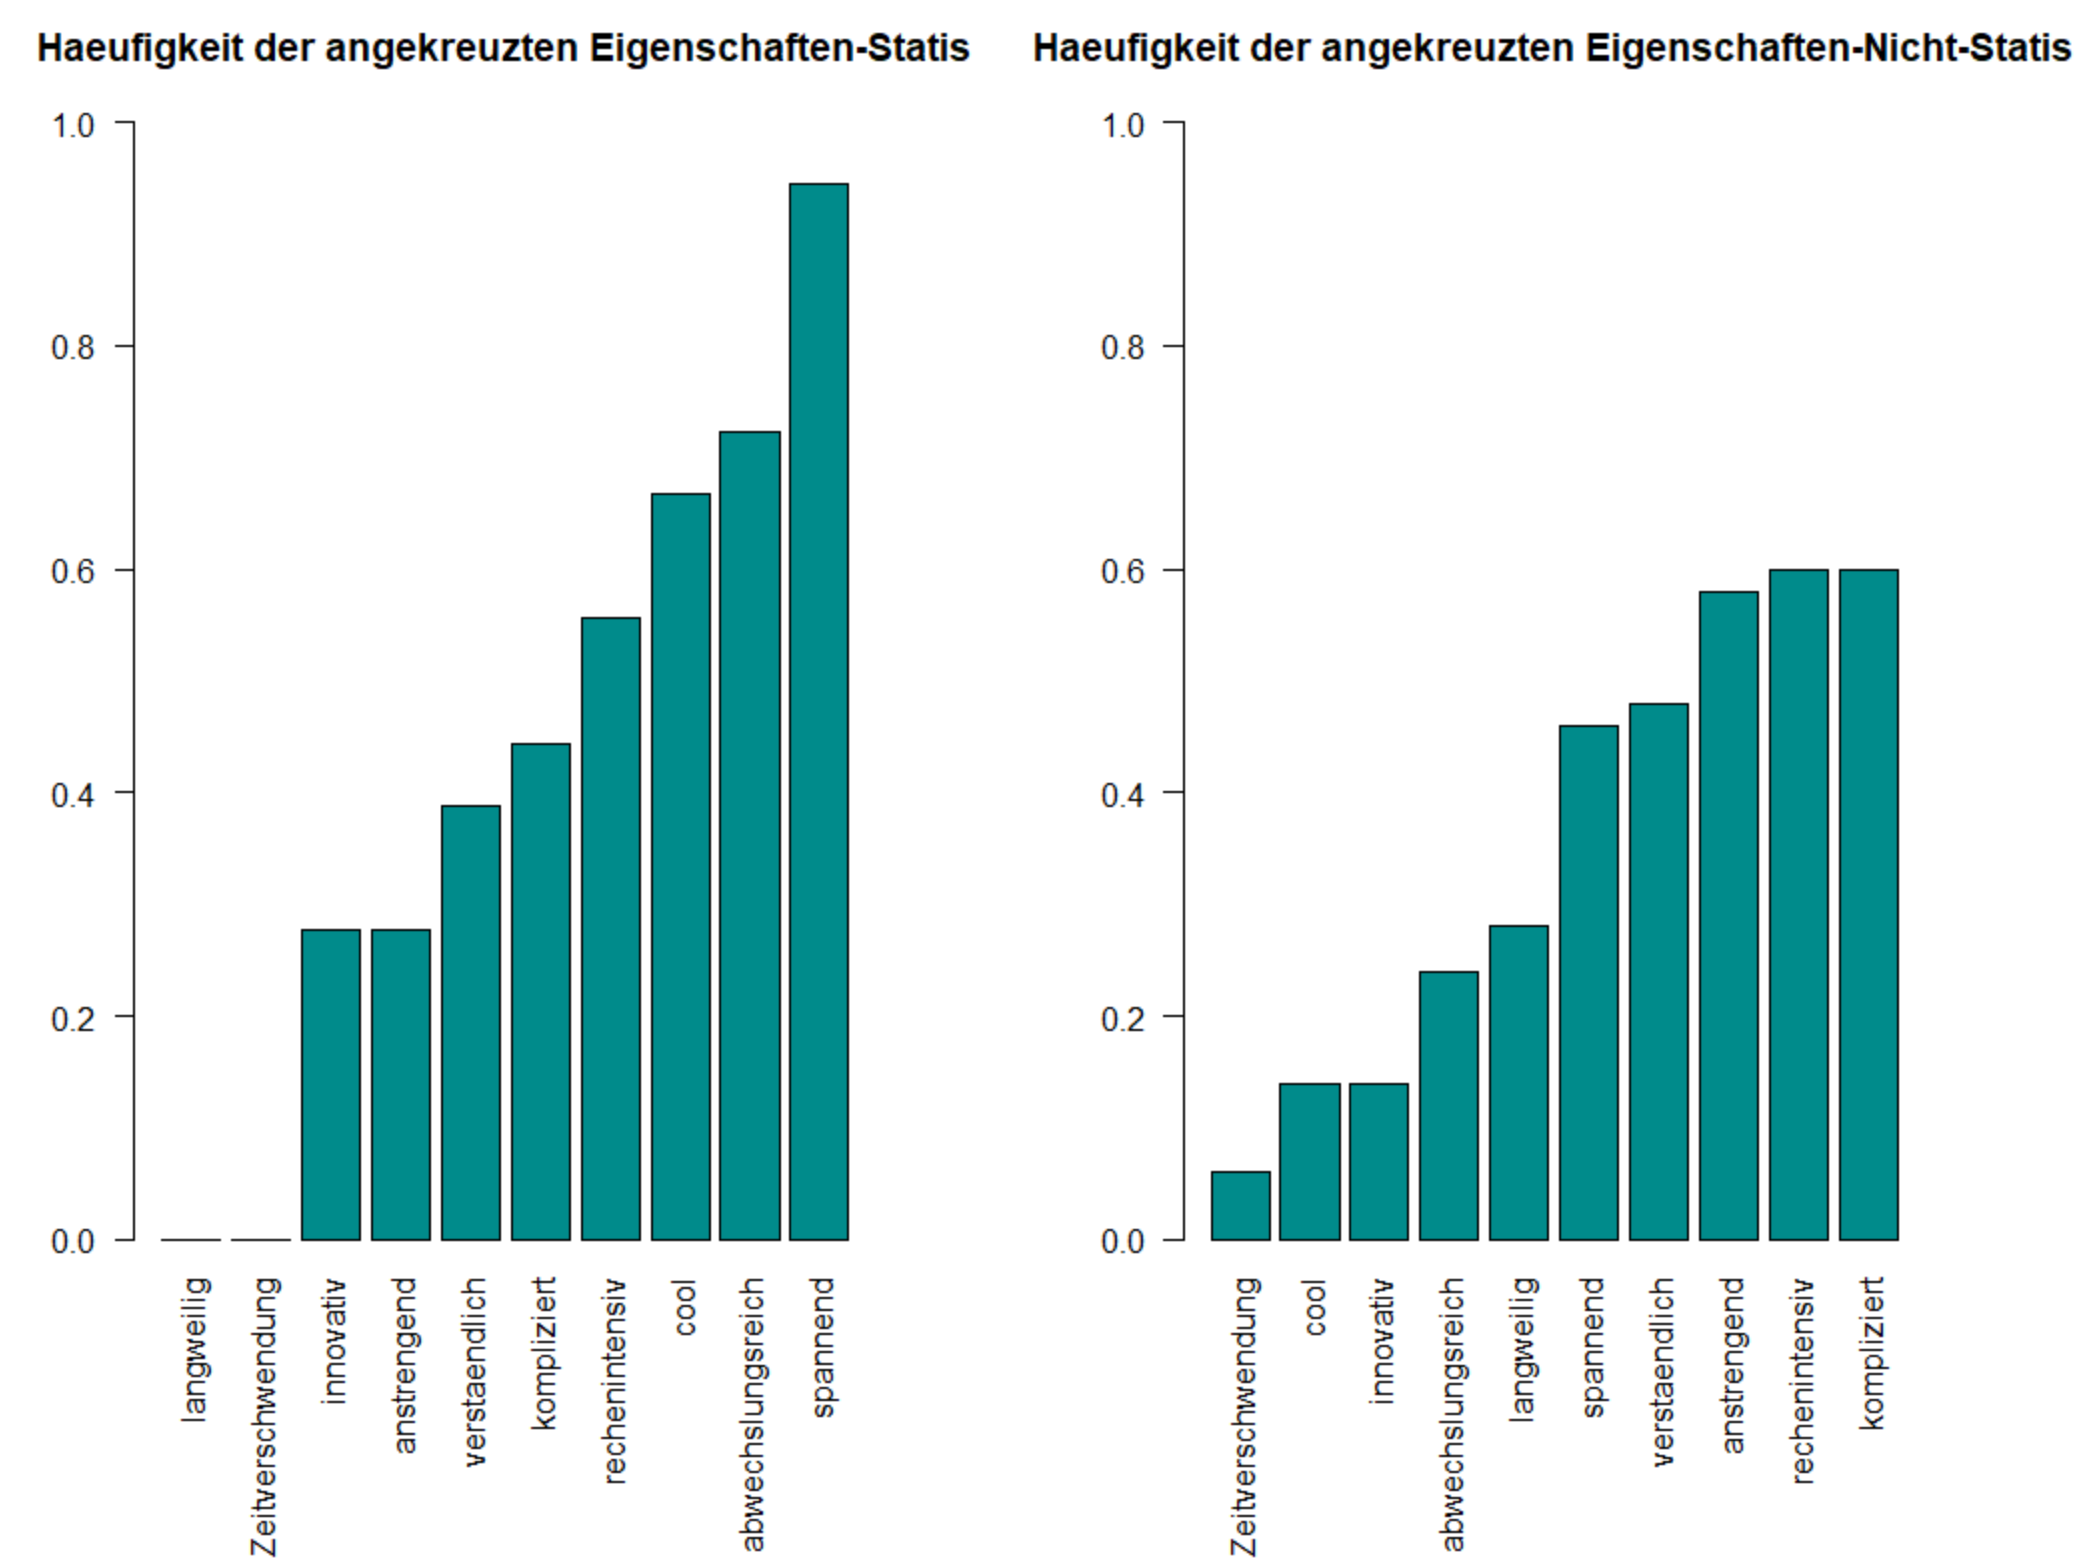
\includegraphics[scale=0.5]{(nicht)-statis_sort_Hfgkeit_angekreuzter_Eigenschaften}
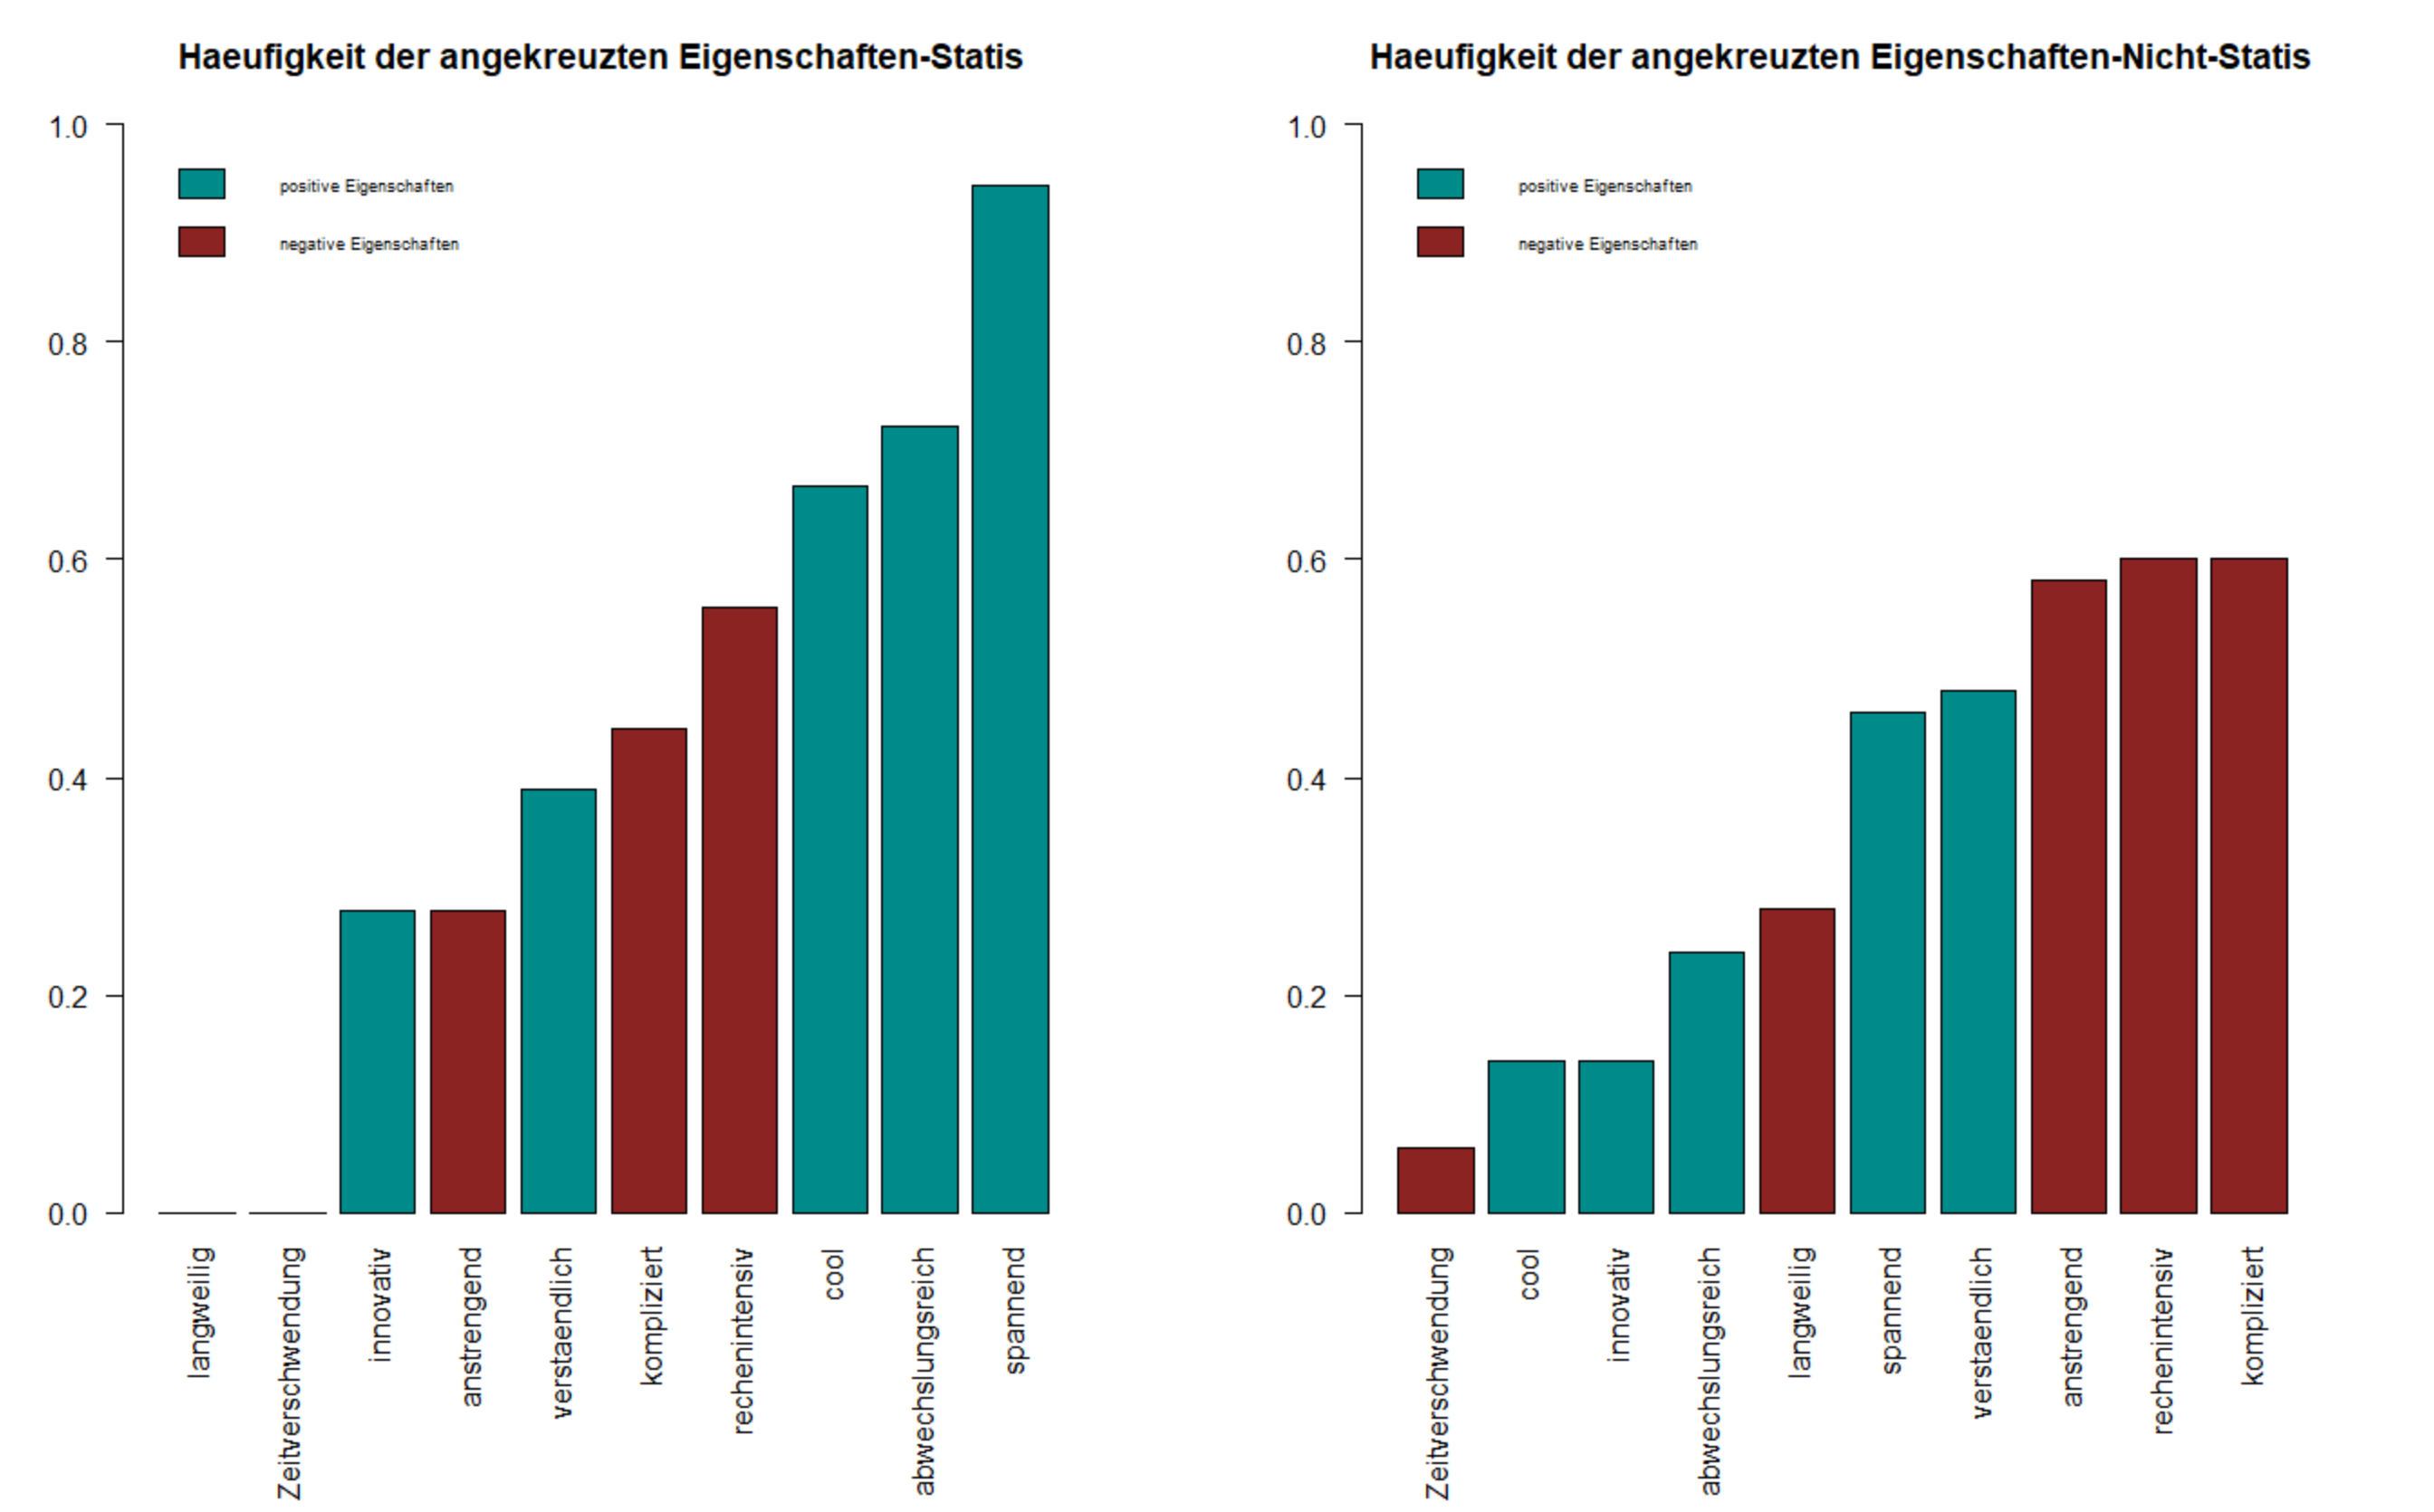
\includegraphics[scale=0.5]{(nicht)-statis_sort_pos_neg_Hfgkeit_angekreuzter_Eigenschaften}\\
\vspace{0.2cm}\\
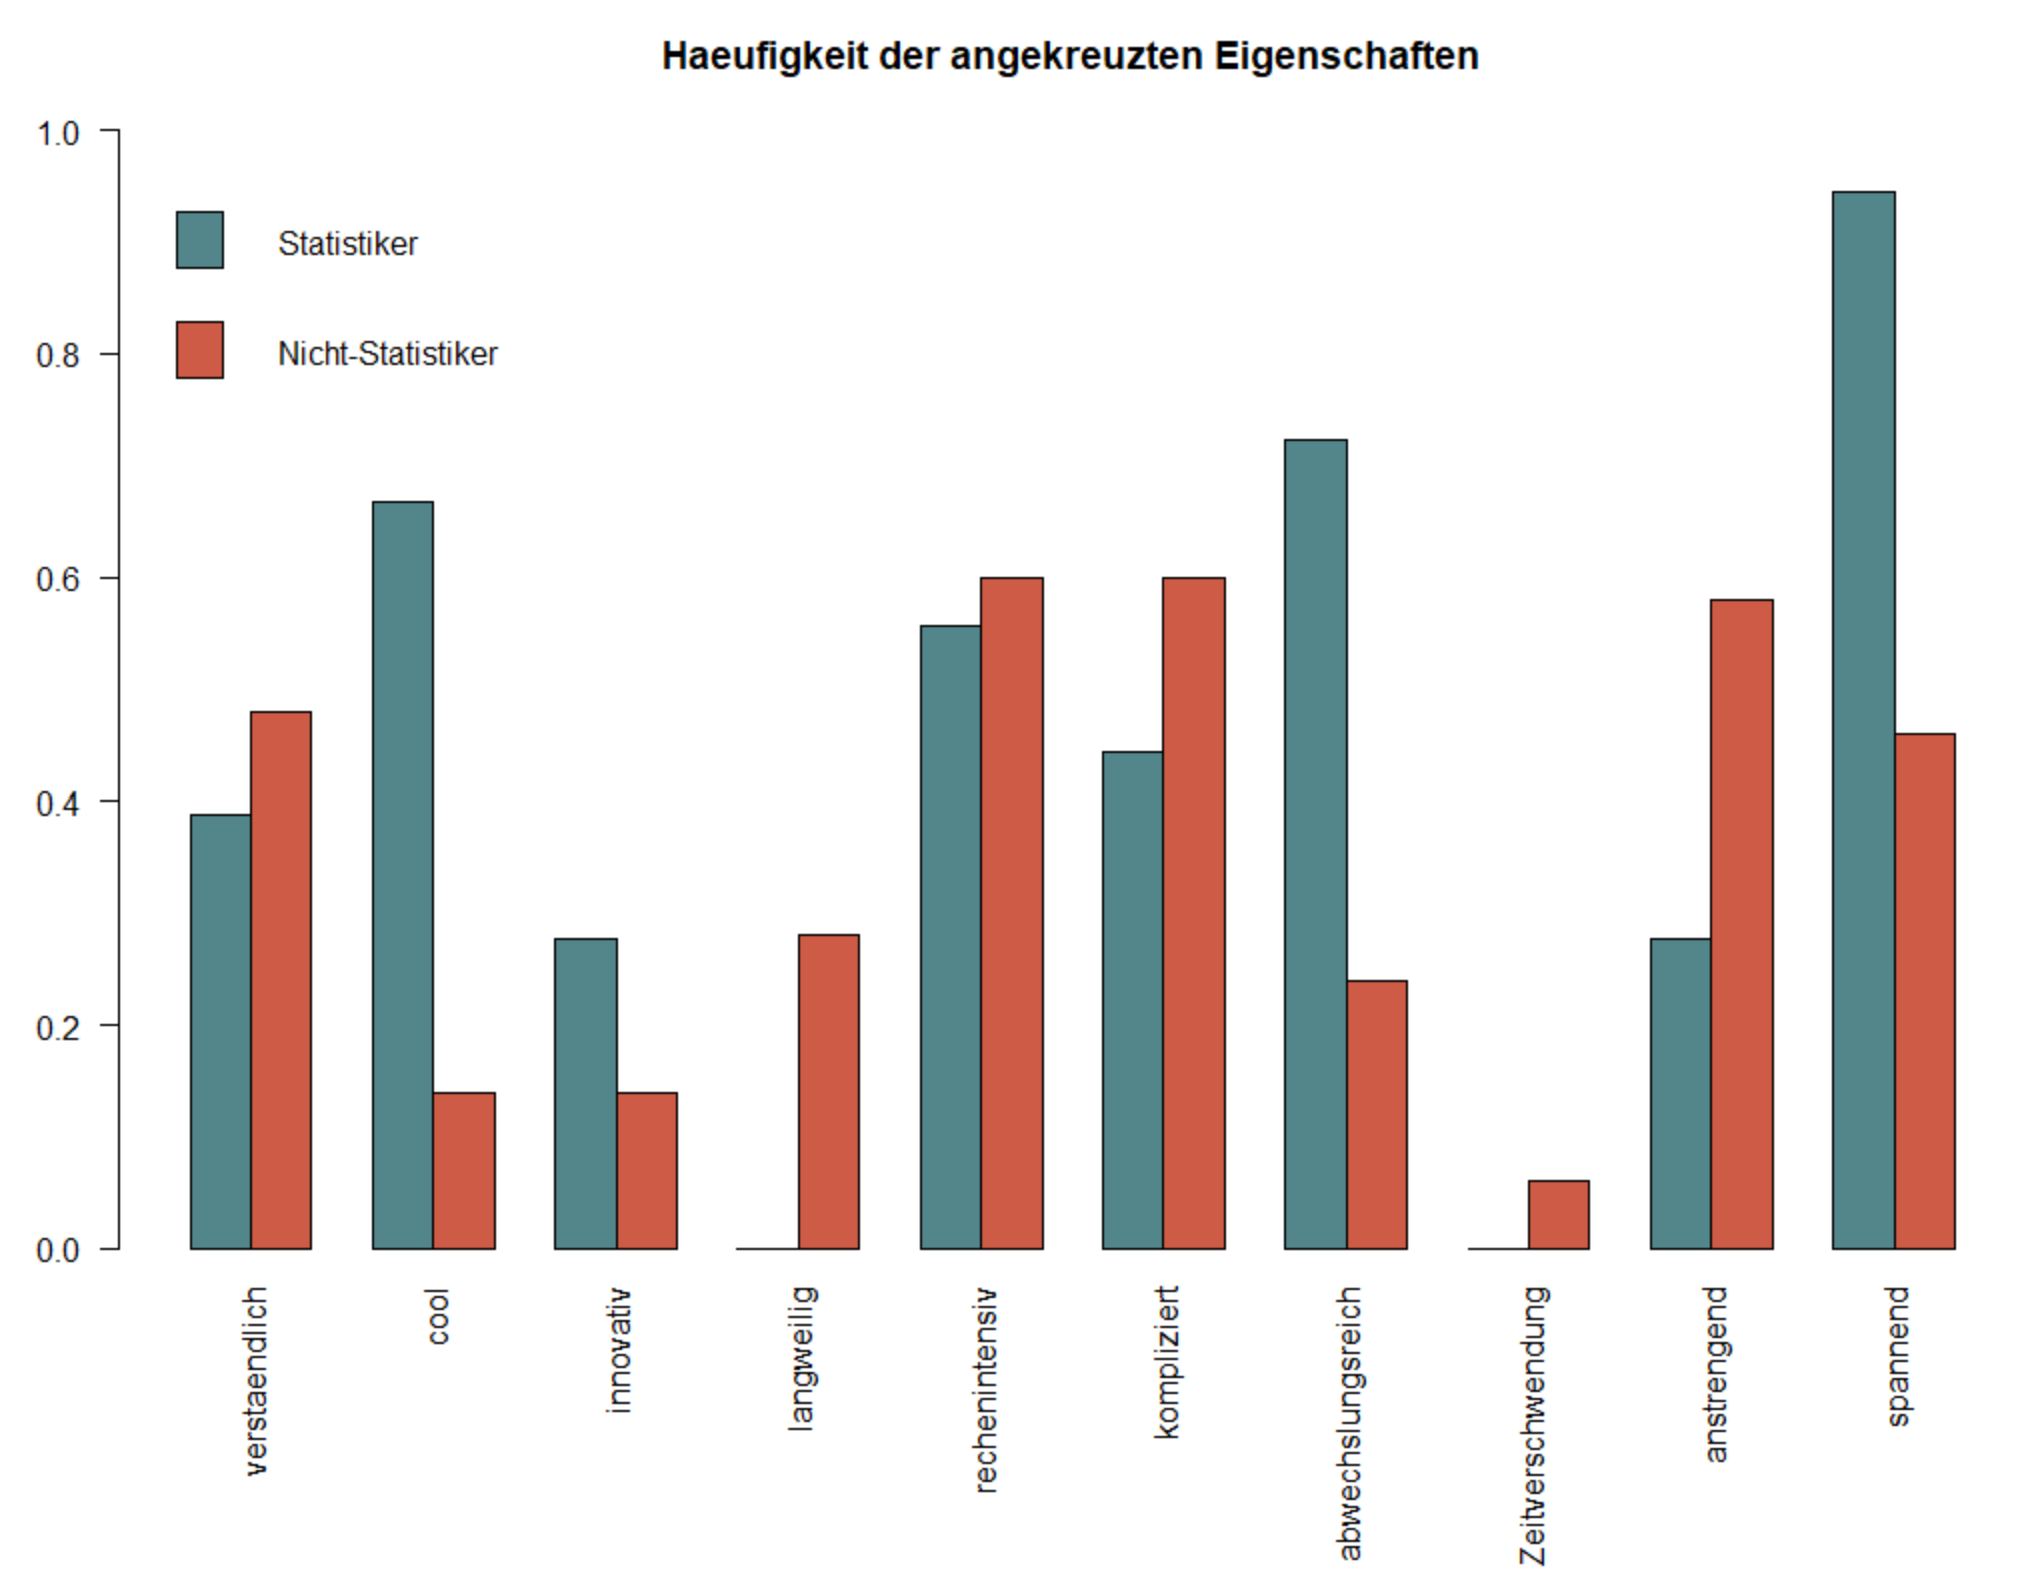
\includegraphics[scale=0.5]{(nicht)-statis_Hfgkeit_angekreuzter_Eigenschaften}\\


%Relevanz:\\
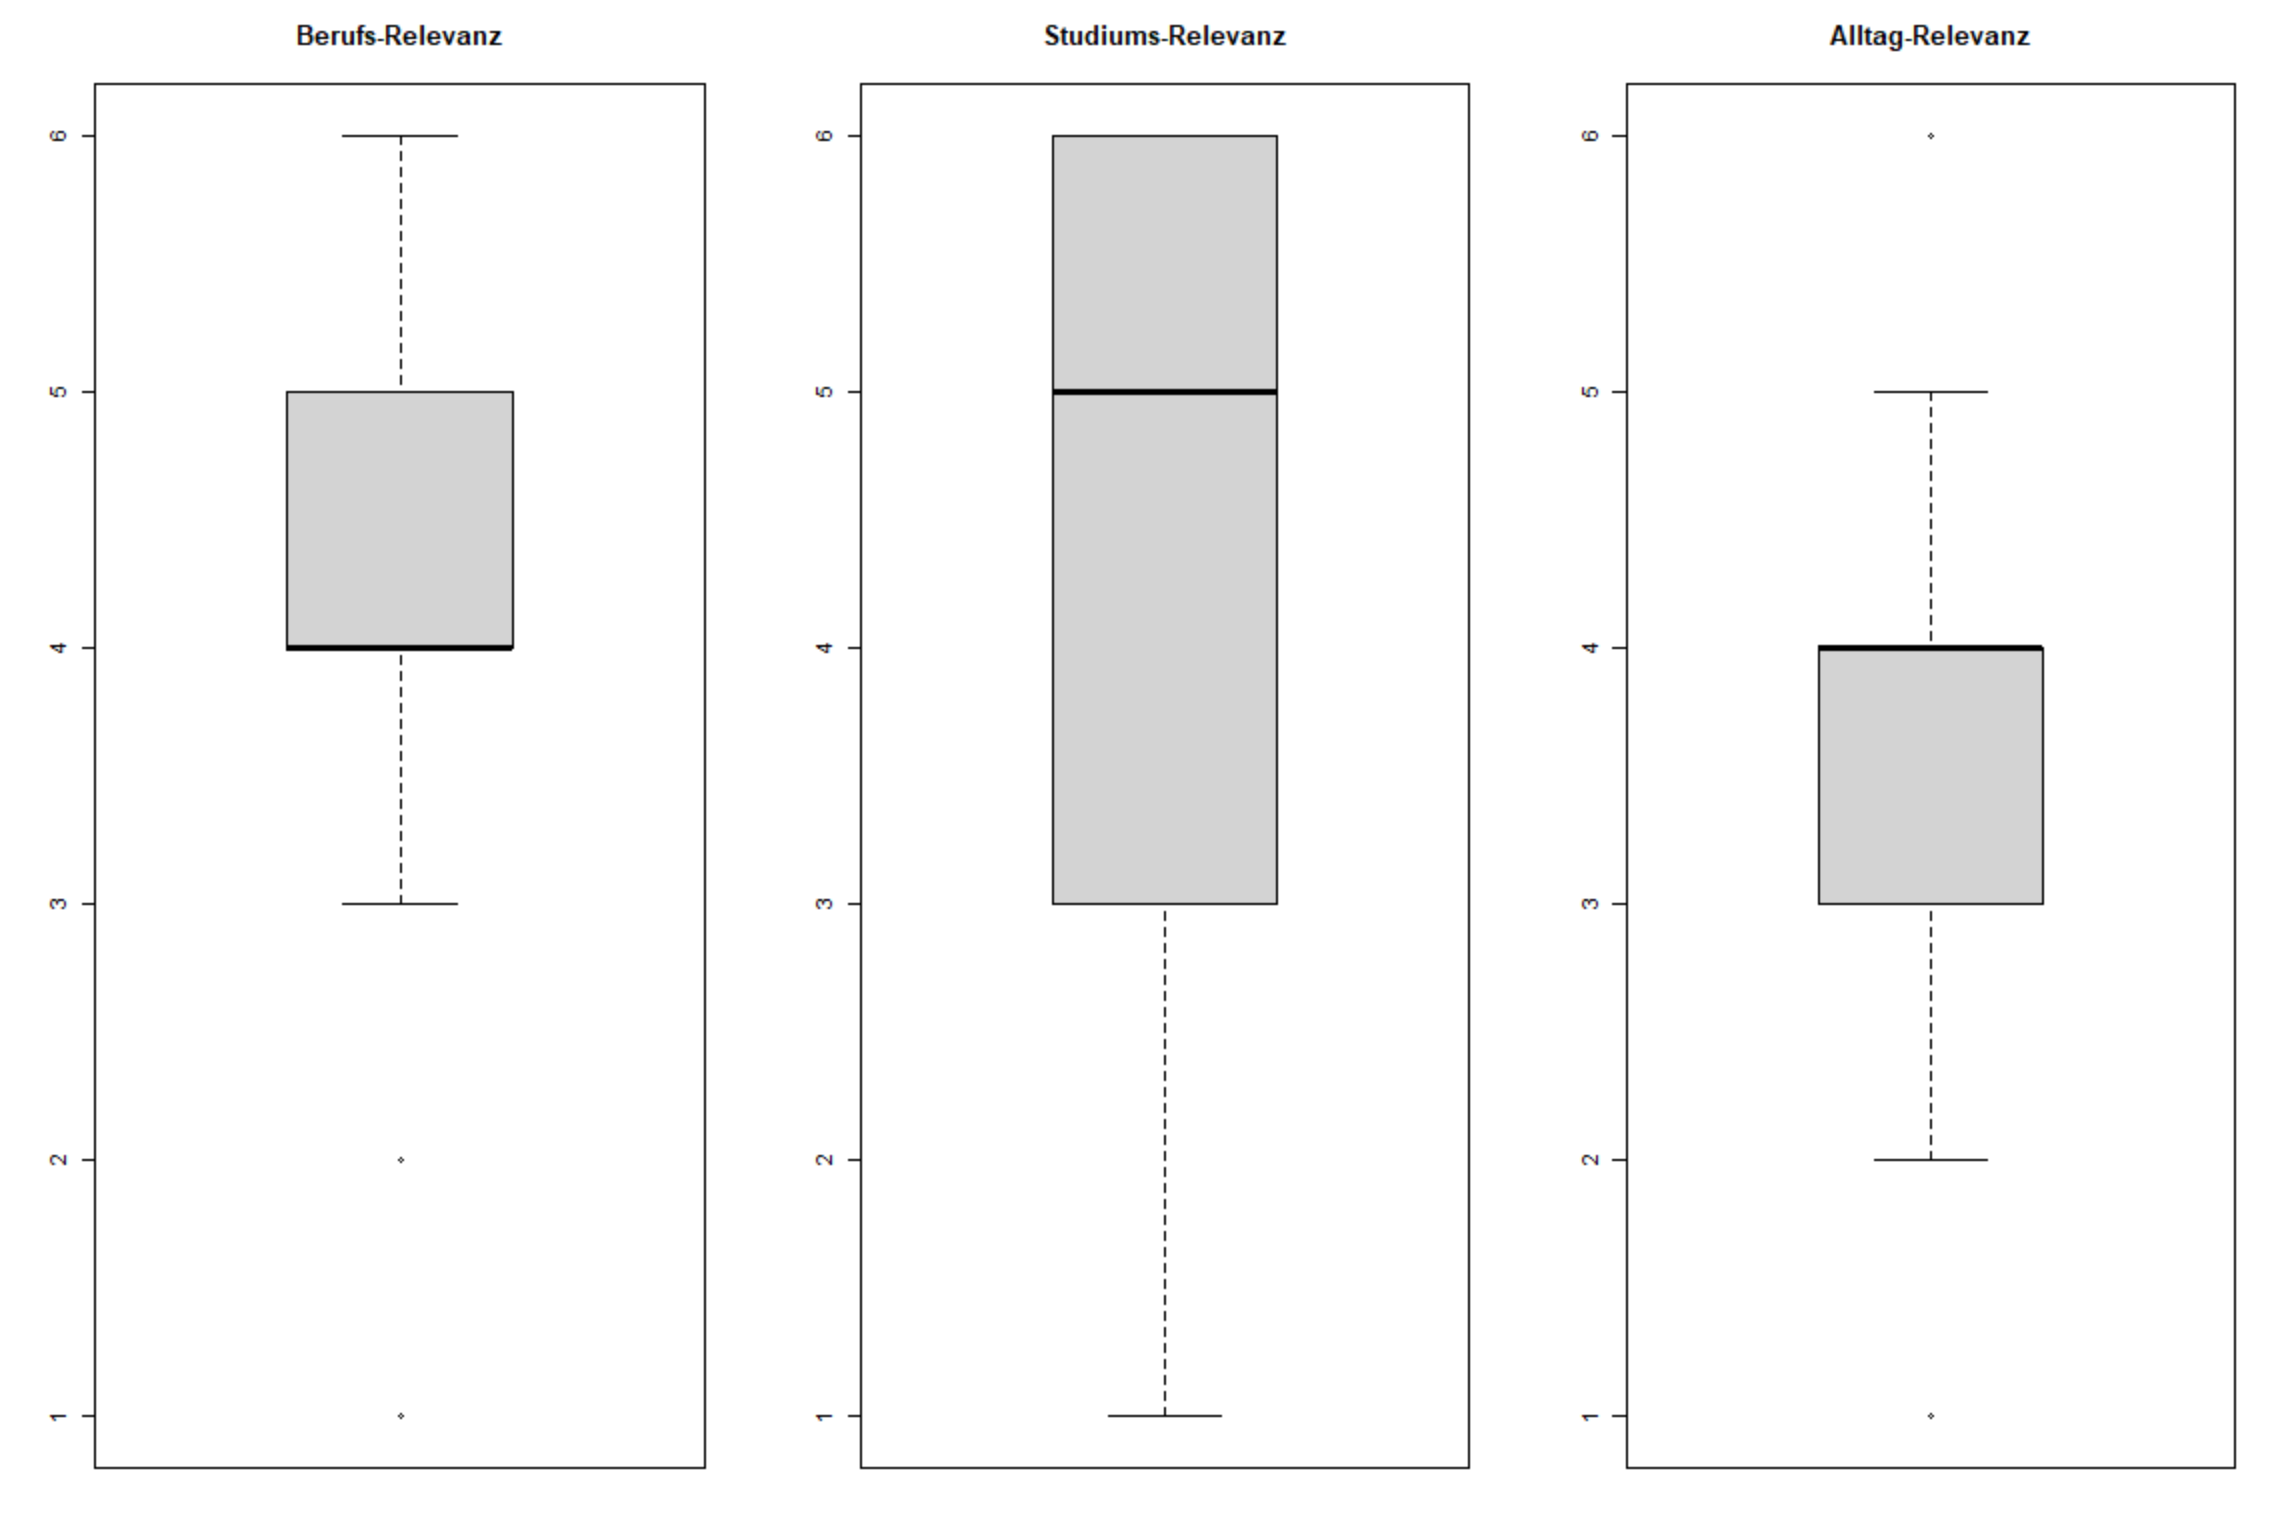
\includegraphics[scale=0.49]{3_boxplots_relevanz}\\
%\vspace{0.1cm}\\
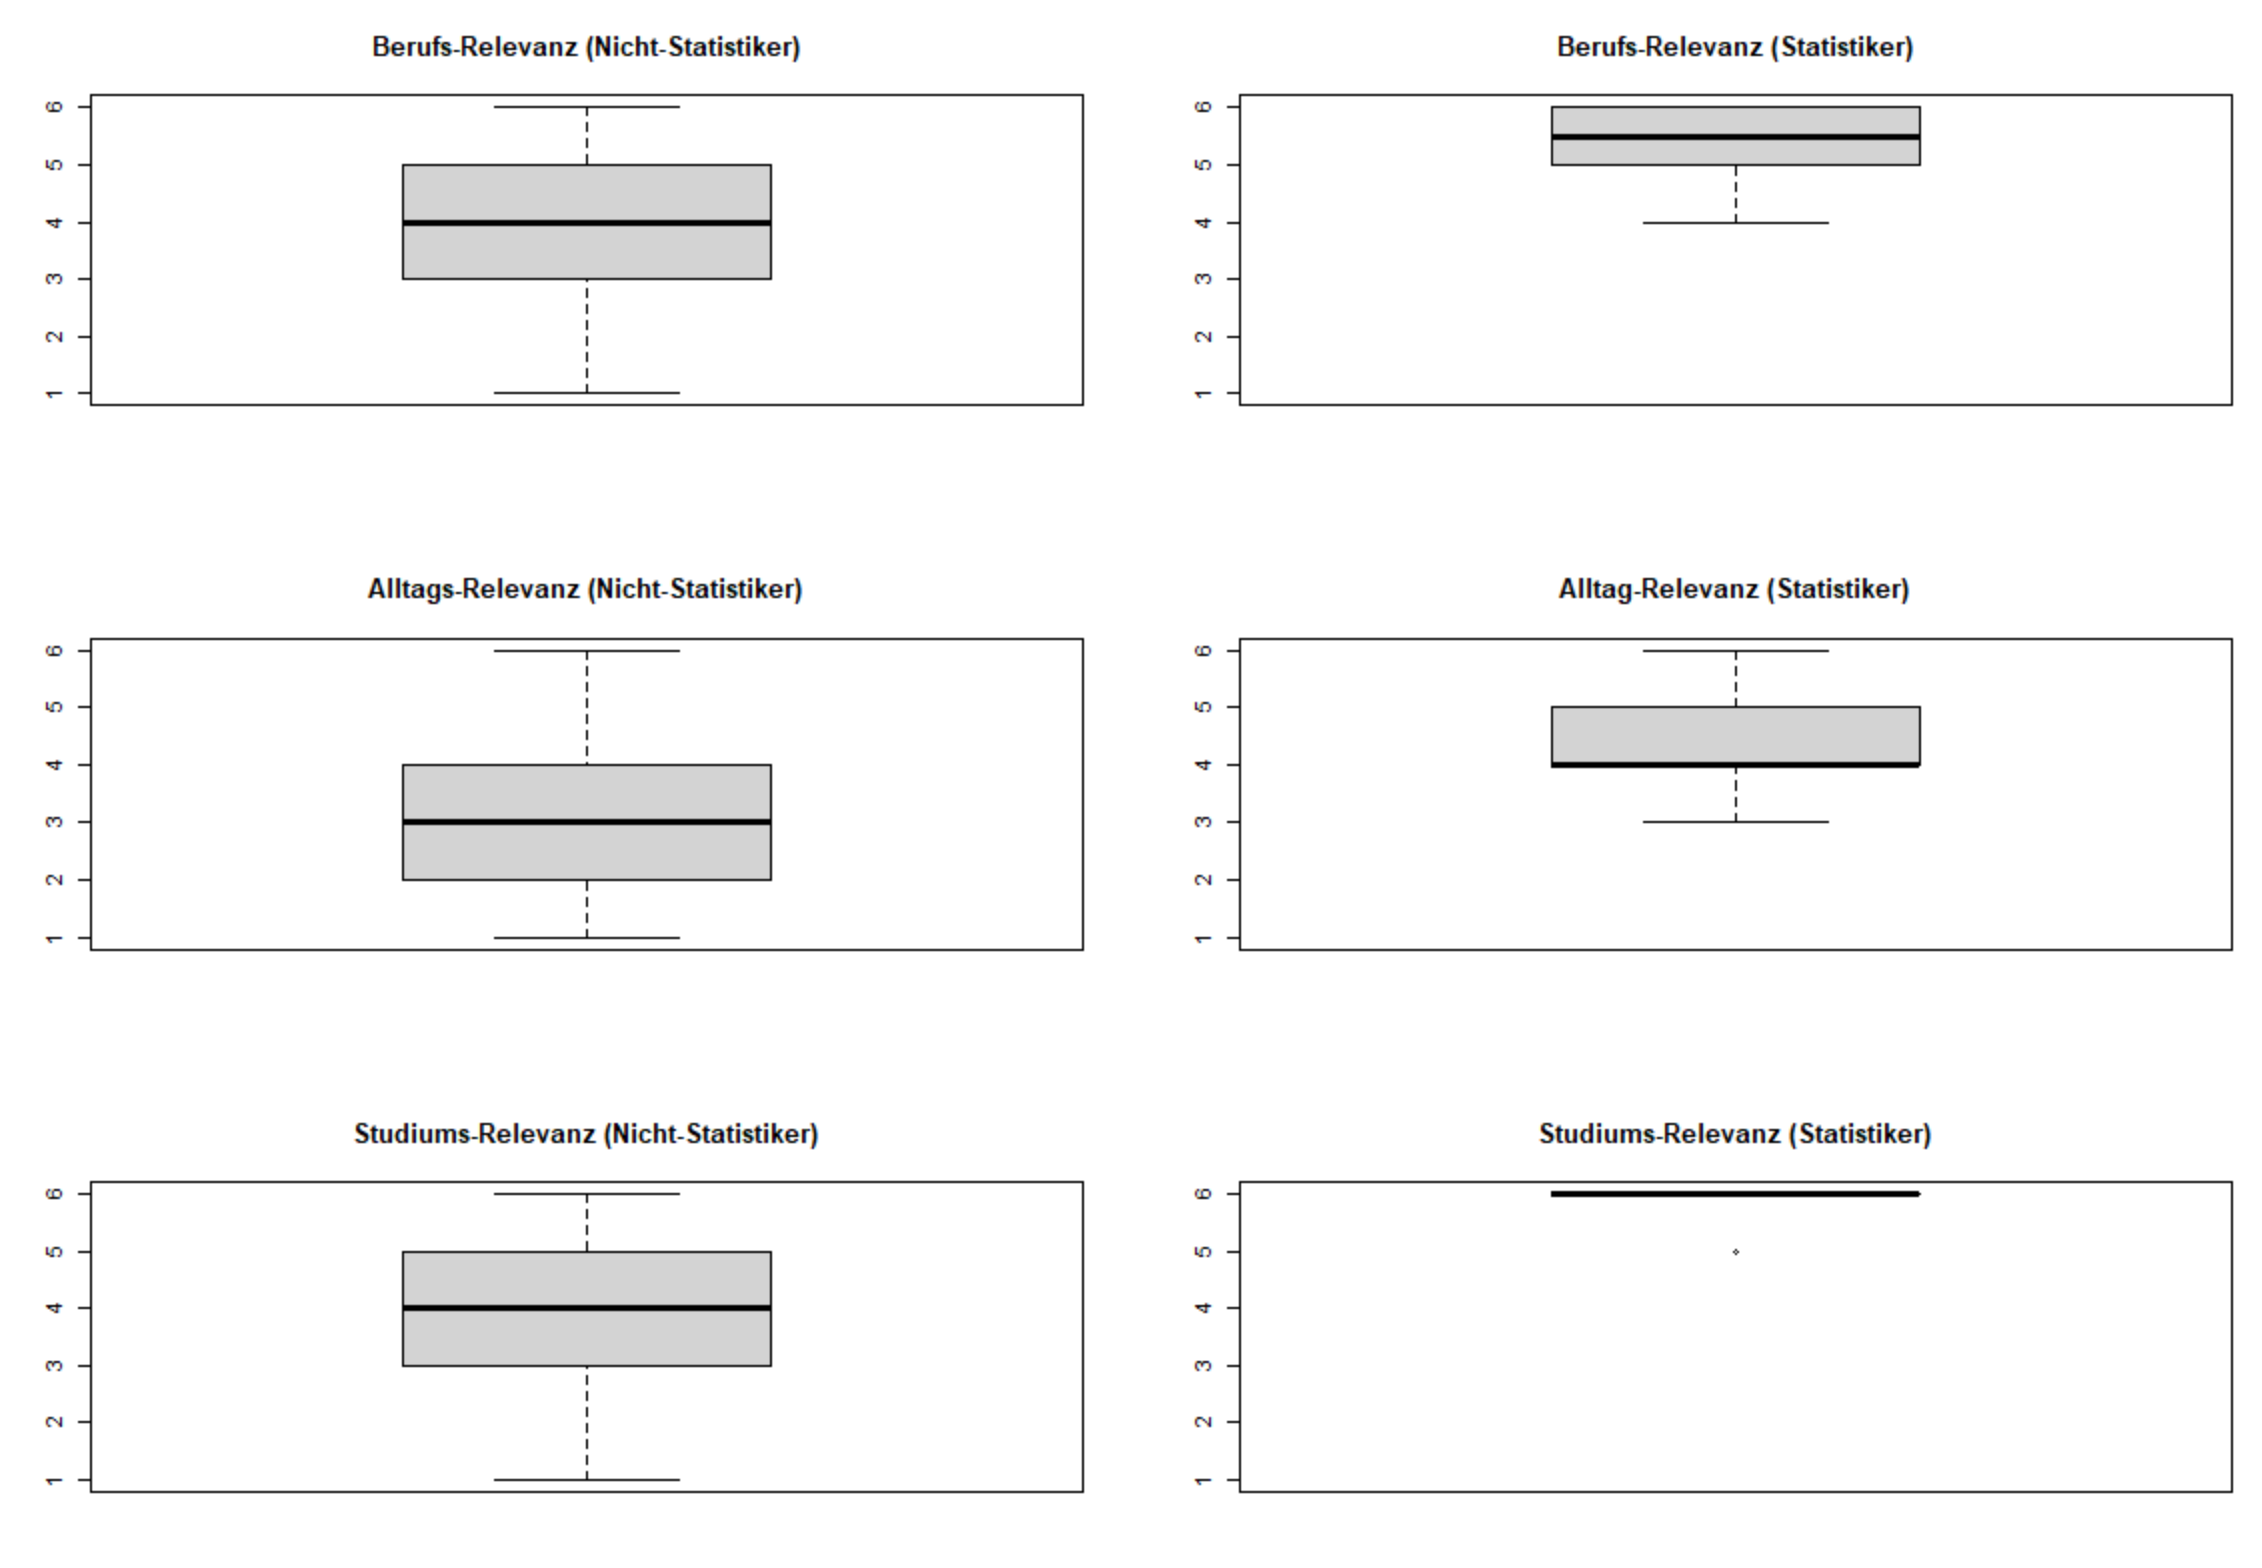
\includegraphics[scale=0.49]{(nicht)-statis_boxplots_Relevanz}\\
{\tiny 1 $=$ Absolut irrelevant, 2 $=$ Ziemlich irrelevant, 3 $=$ Eher irrelevant, 4 $=$ Eher relevant, 5 $=$ Ziemlich relevant, 6 $=$ Absolut relevant}\\


%Assoziationen:\\
\hspace{-2cm}
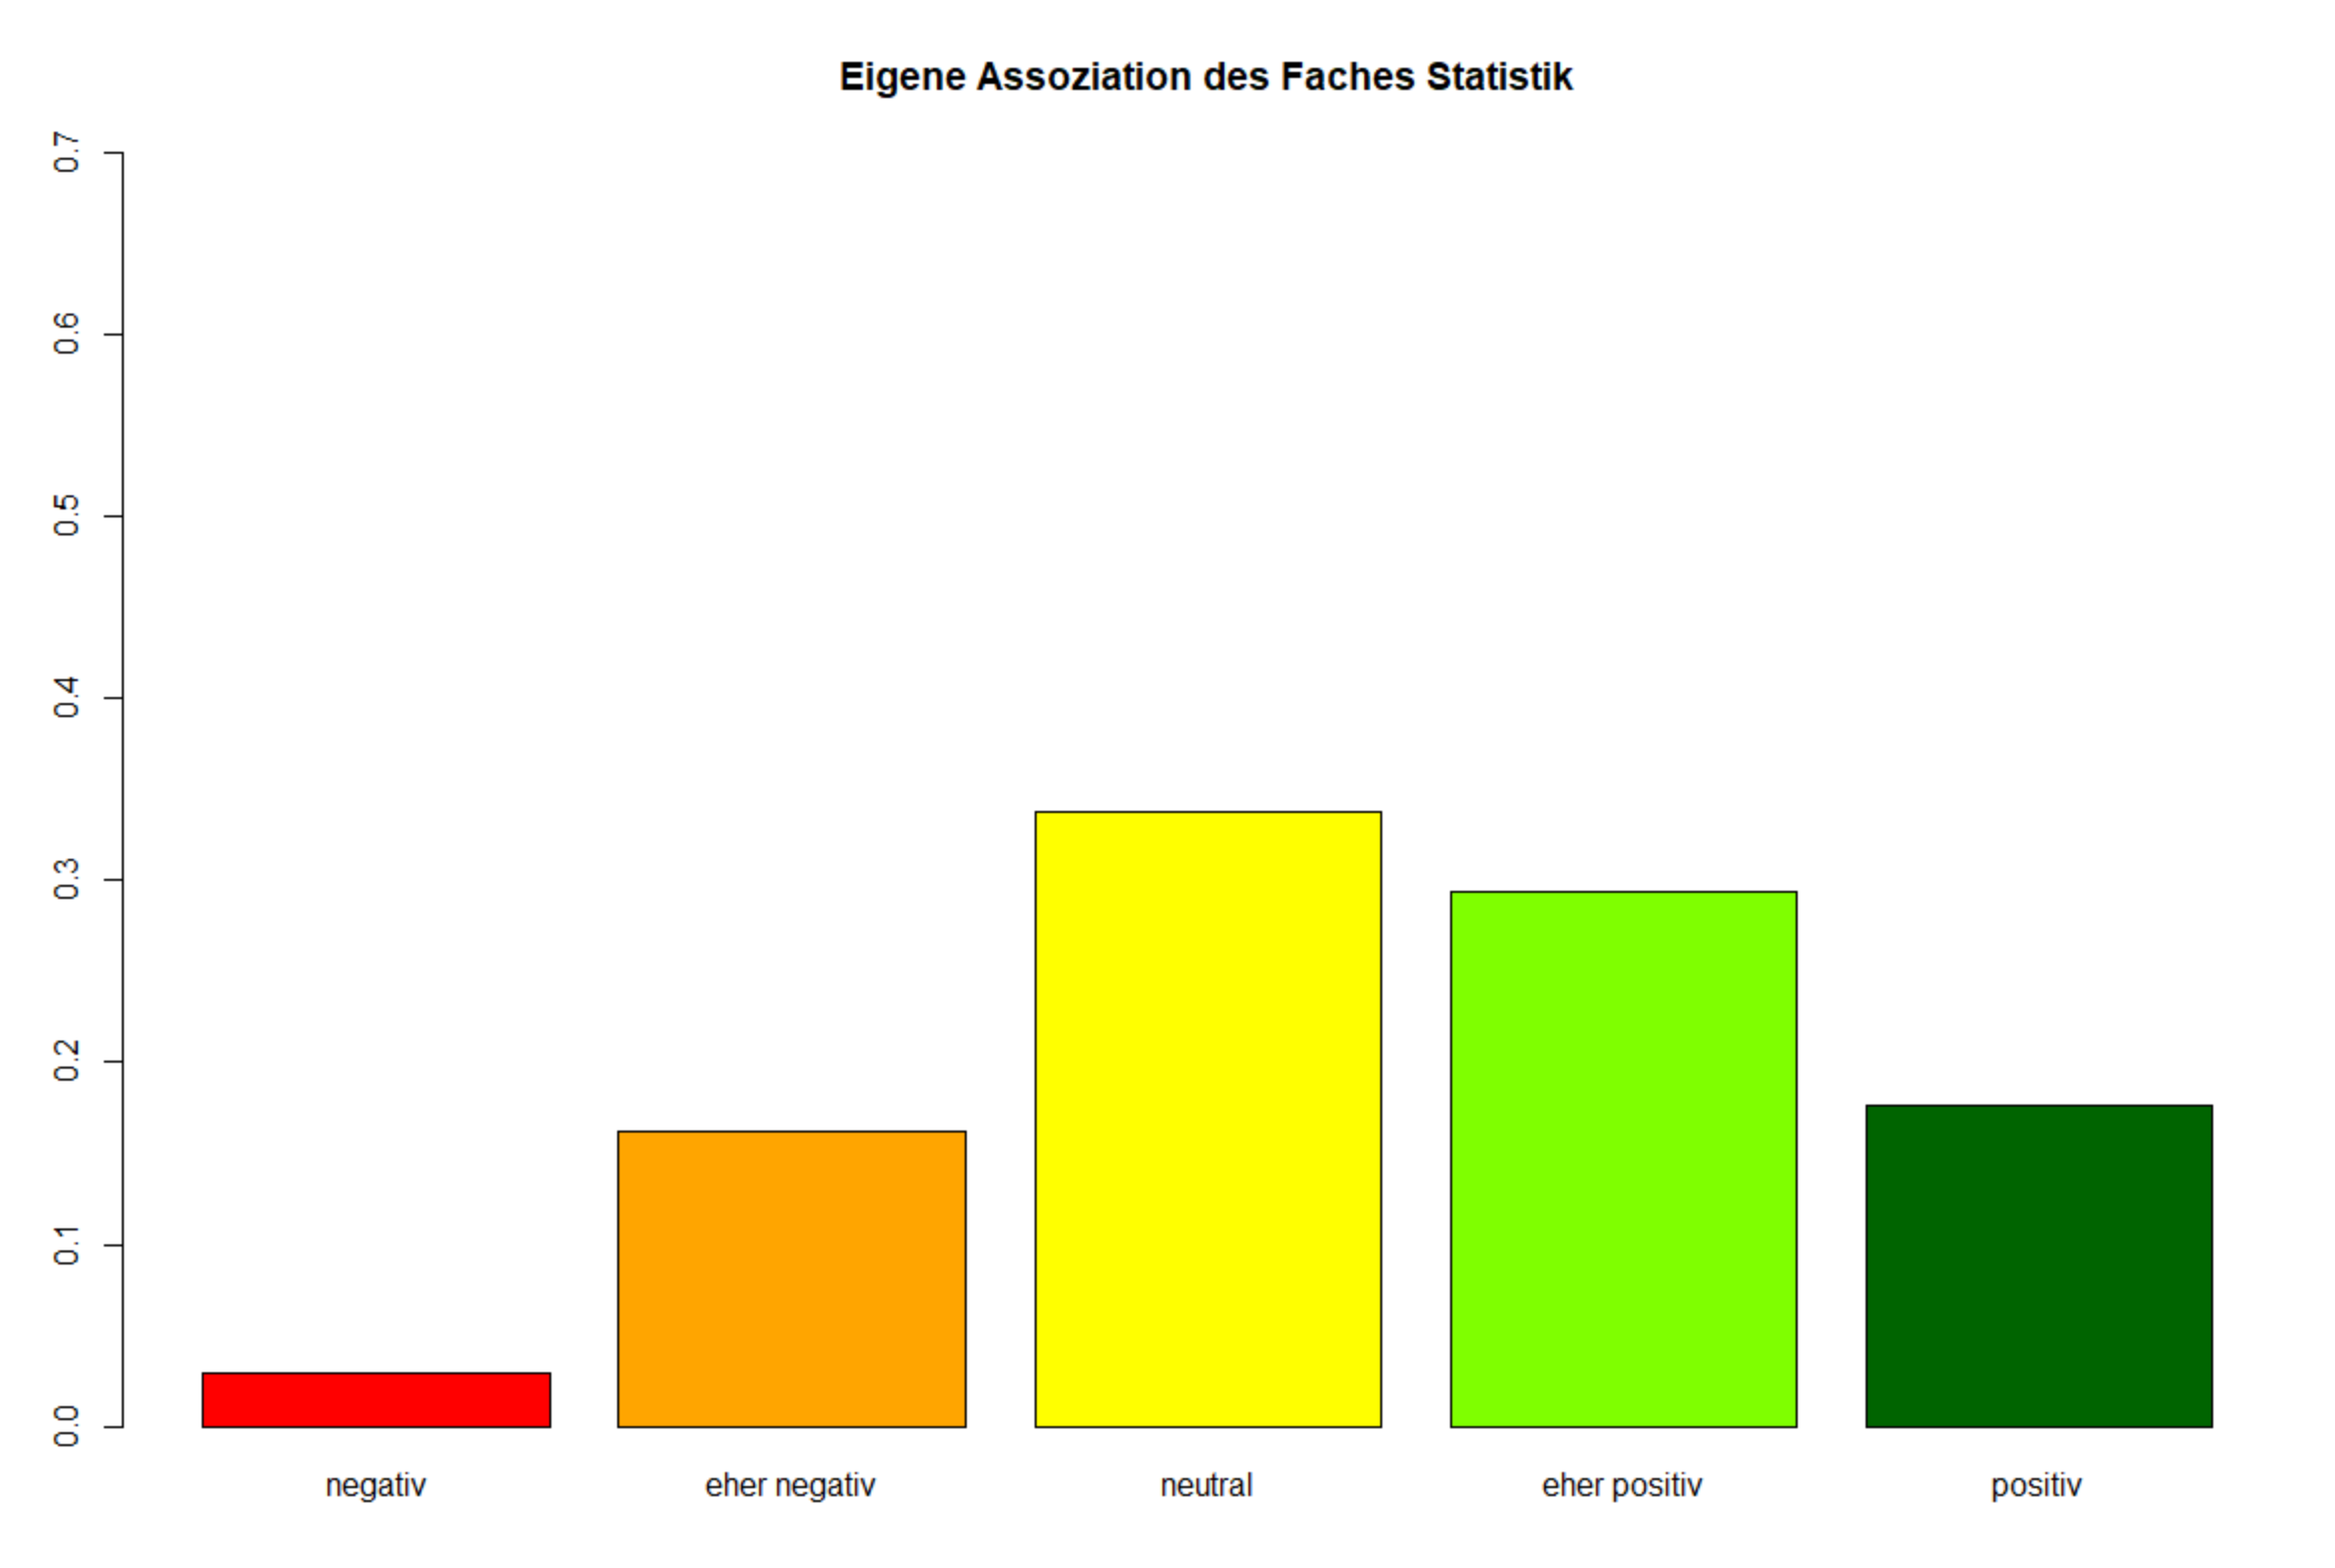
\includegraphics[scale=0.3]{barplot_Assoziation}
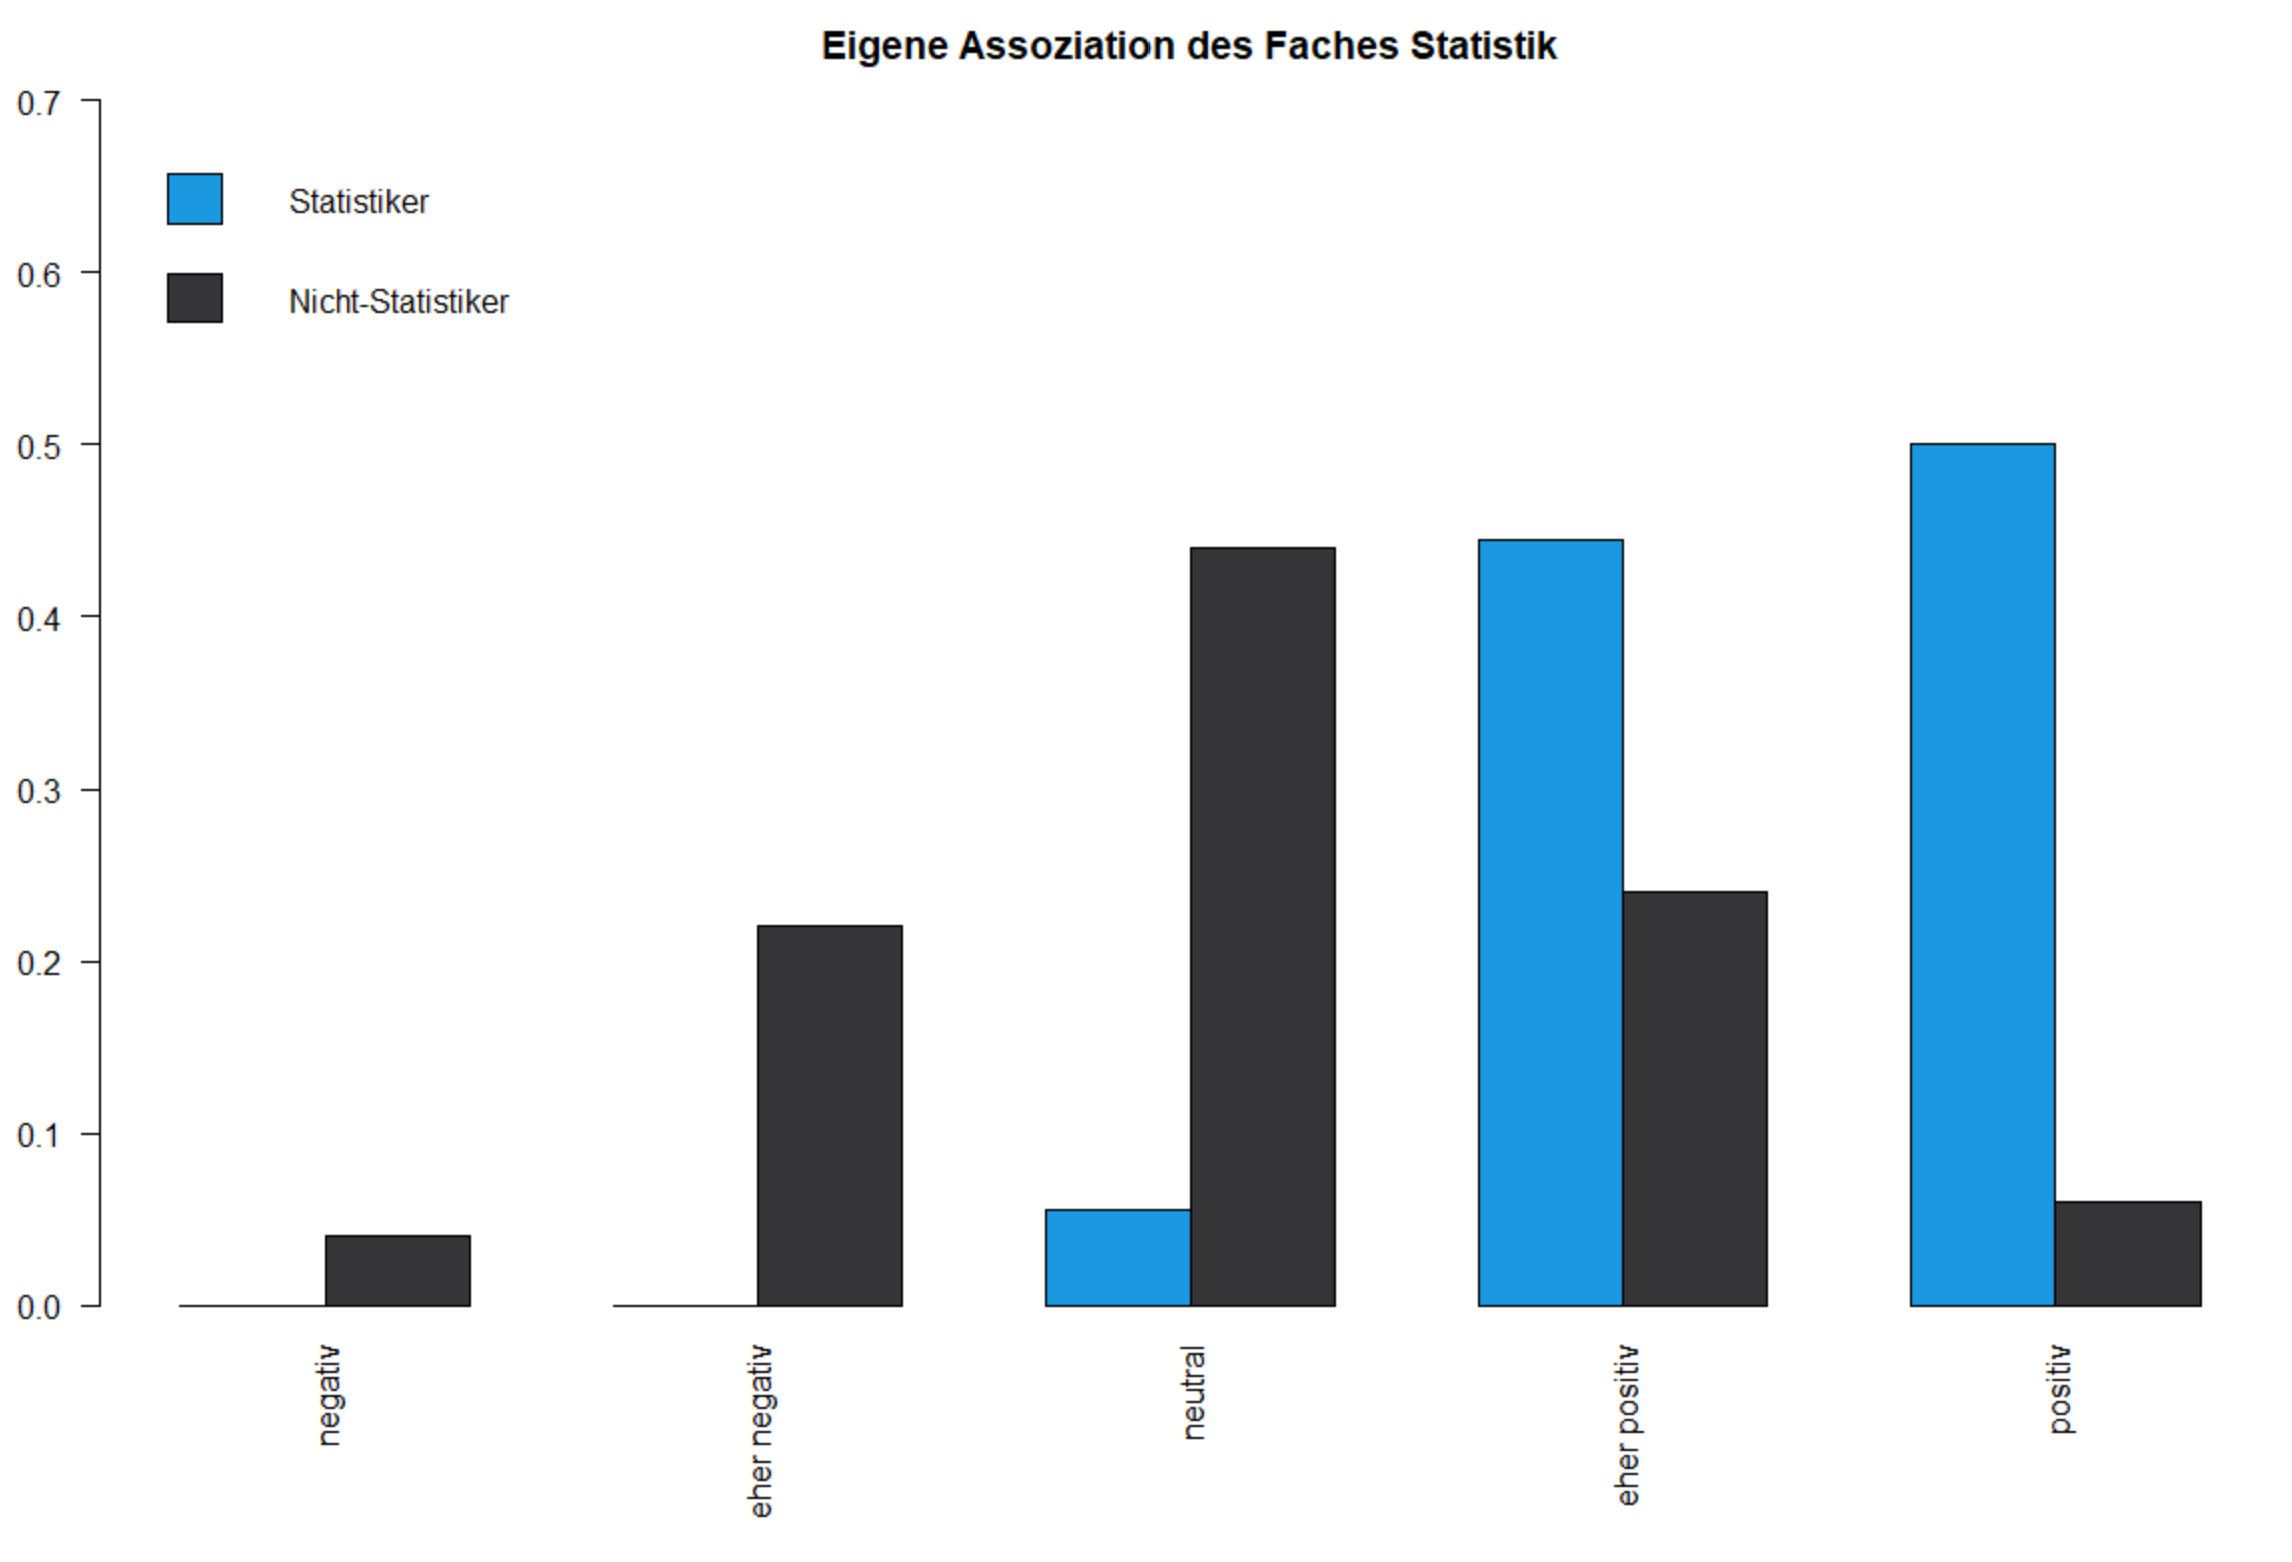
\includegraphics[scale=0.3]{(nicht)-statis_barplot_Assoziation} \\


%Wahrnehmung:\\
\hspace{-2cm}
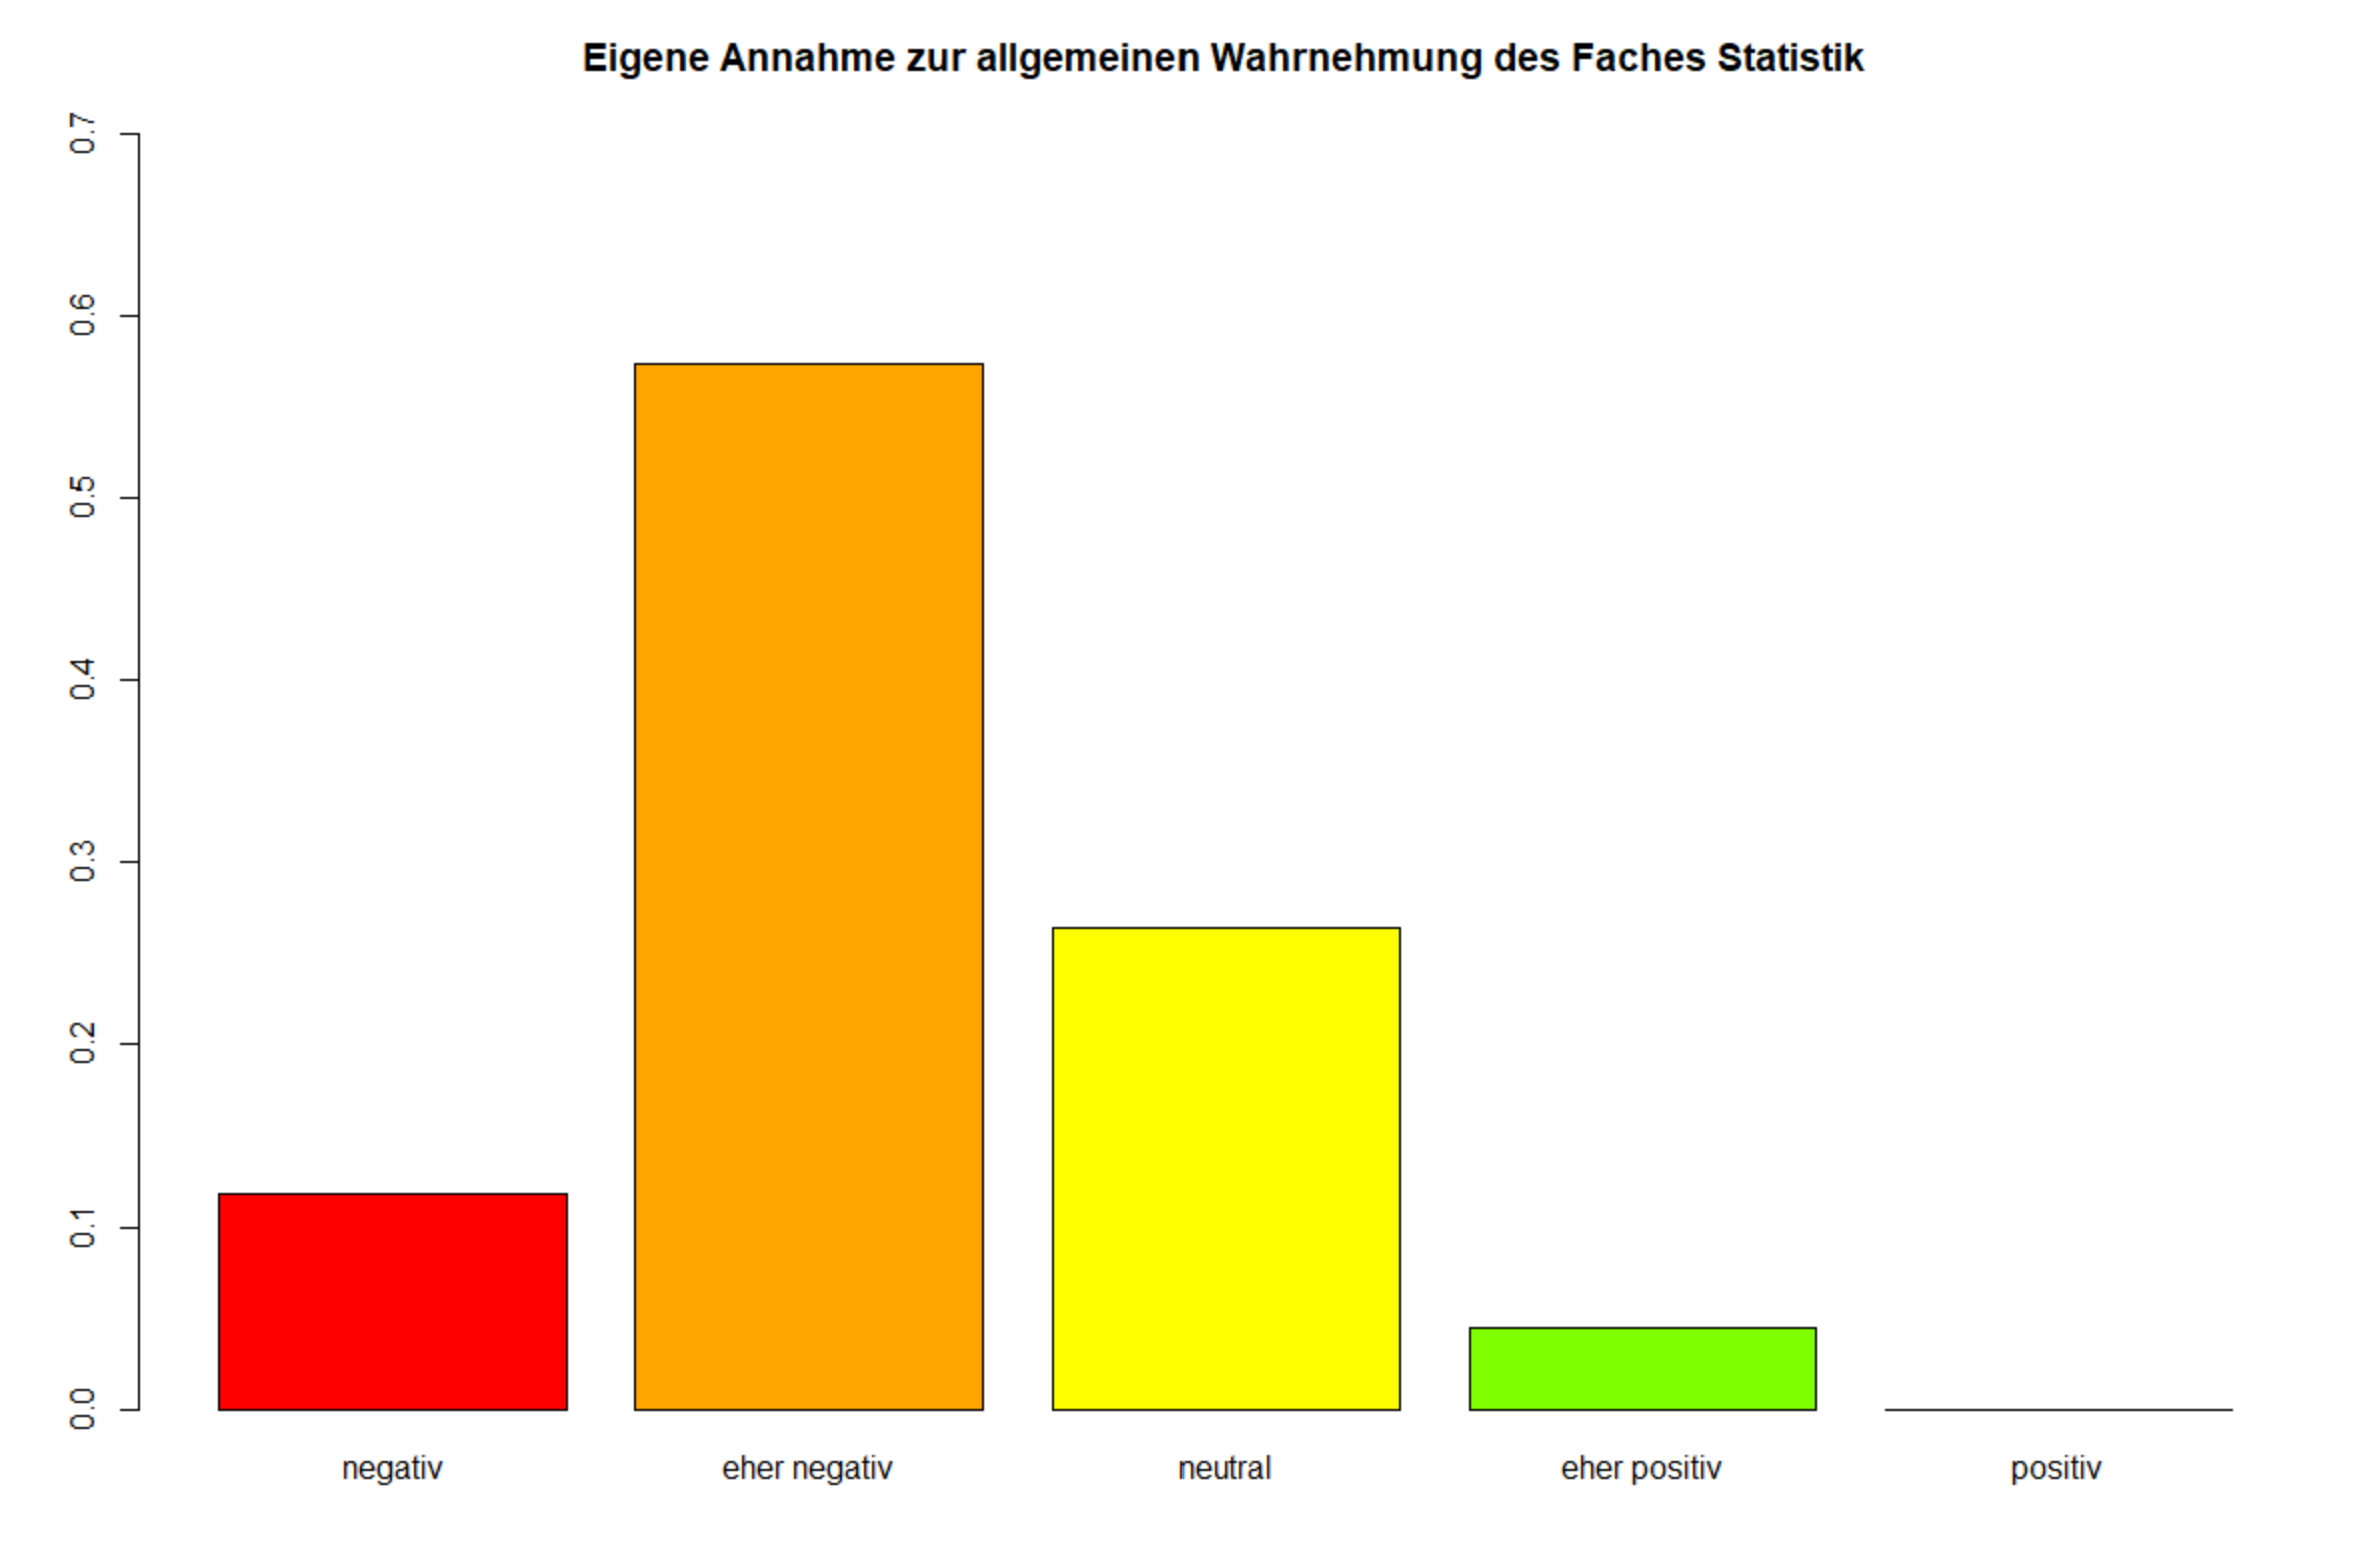
\includegraphics[scale=0.3]{barplot_Wahrnehmung}
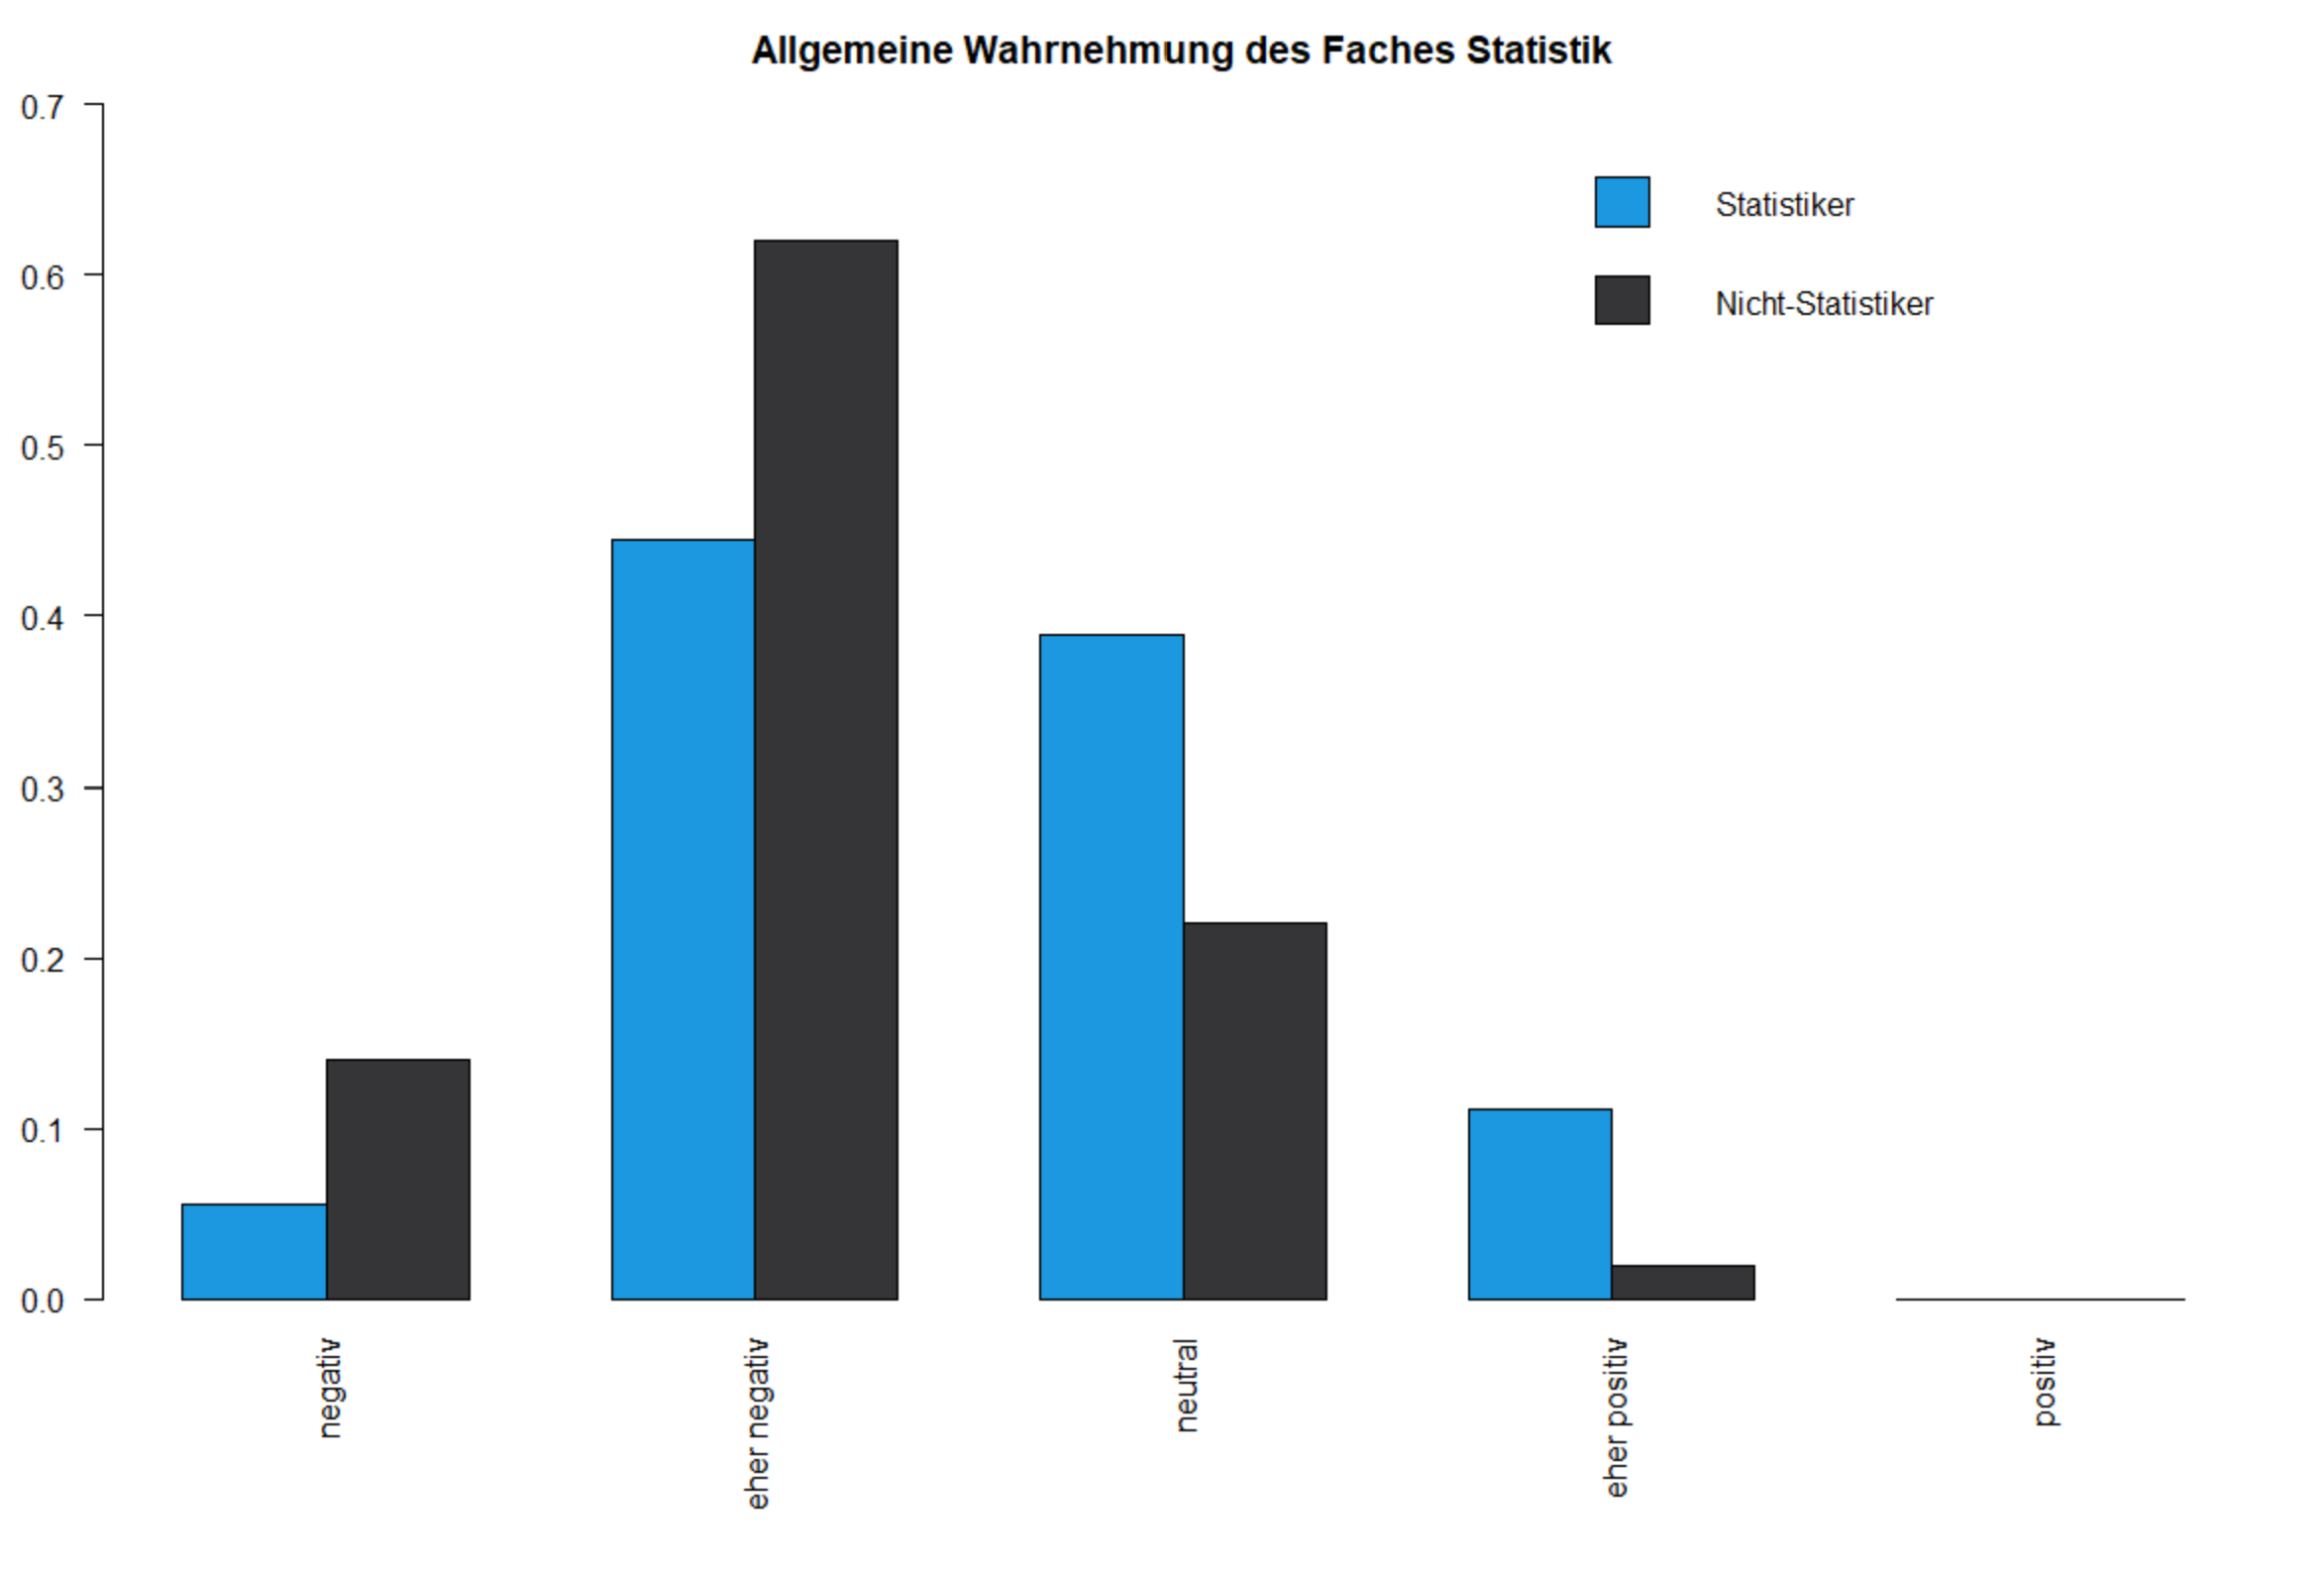
\includegraphics[scale=0.3]{(nicht)-statis_barplot_Wahrnehmung}\\

\vspace{-0.4cm}

%Text zur Forschungsfrage:\\
{\small Bis auf die Thesen \enquote{Statistiken beweisen gar nichts}, \enquote{Statistik fördert Kreativität} und \enquote{Statistik studieren nur Männer} gab es zu allen Thesen eine ziemlich eindeutige Zustimmung oder Ablehnung.\\
Negative Eigenschaften zu Beschreibung des Fachs Statistik wurden deutlich häufiger von Nicht-Statistikern angekreuzt, während die Statistiker mehr positive angekreuzt haben.\\
Besonders relevant war die Statistik für die Befragten im Studium und tendenziell im zukünftigen Beruf, jedoch weniger im Alltag. Die befragten Statistikern haben im Mittel eine höhere Relevanz für alle 3 Bereiche angegeben im Vergleich zu den Nicht-Statistikern.\\
Nicht-Statistiker haben im Mittel neutrale und Statistiker ziemlich positive Assoziationen zum Fach Statistik, was zu einer neutralen bis tendenziell positiven Assoziation im Allgemeinen führt.\\
Dennoch wird im Allgemeinen angenommen, dass die Statistik eher negativ wahrgenommen werden würde, wobei keiner der Befragten angab, dass die Wahrnehmung in der Gesellschaft \enquote{positiv} wäre.}

\section{Anhang: Tabellen mit Anteilwerten und Korrelationen}

\subsection{Thesen (gesamt)}
  \begin{table}[ht]
 
\begin{tabular}{rrrr}
  \hline
 & Traue\_keiner\_Statistik & zukunftsorientiert & trocken \\ 
  \hline
Stimme gar nicht zu & 0.08 & 0.07 & 0.03 \\ 
  Stimme eher nicht zu & 0.35 & 0.18 & 0.39 \\ 
  Stimme eher zu & 0.34 & 0.41 & 0.41 \\ 
  Stimme voll zu & 0.23 & 0.34 & 0.17 \\ 
   \hline
\end{tabular}

\bigskip

\begin{tabular}{rrrr}
  \hline
 & gute\_Berufsaussichten & Angst & wichtige\_Informationsquelle \\ 
  \hline
Stimme gar nicht zu & 0.04 & 0.03 & 0.01 \\ 
  Stimme eher nicht zu & 0.08 & 0.13 & 0.07 \\ 
  Stimme eher zu & 0.35 & 0.41 & 0.38 \\ 
  Stimme voll zu & 0.52 & 0.44 & 0.54 \\ 
   \hline
\end{tabular}

\bigskip 

\begin{tabular}{rrrr}
  \hline
 & nur\_Maenner & Kreativitaet & beweisen\_nichts \\ 
  \hline
Stimme gar nicht zu & 0.59 & 0.28 & 0.38 \\ 
  Stimme eher nicht zu & 0.32 & 0.49 & 0.45 \\ 
  Stimme eher zu & 0.08 & 0.17 & 0.10 \\ 
  Stimme voll zu & 0.00 & 0.06 & 0.07 \\ 
   \hline
\end{tabular}

\bigskip

\begin{tabular}{rrr}
  \hline
 & vielfaeltige\_Anwendungsgebiete \\ 
  \hline
Stimme gar nicht zu & 0.01 \\ 
  Stimme eher nicht zu & 0.03 \\ 
  Stimme eher zu & 0.23 \\ 
  Stimme voll zu & 0.73 \\ 
   \hline
\end{tabular}
\end{table}
\newpage

\subsection{Korrelationen Thesen (gesamt)}
\begin{table}[ht]
\begin{tabular}{rrrrrr}
  \hline
 & Tr\_kS & Zuknftor & trocken & Berufaus & Angst \\ 
  \hline
Tr\_kS & 1.00 & -0.20 & 0.02 & 0.03 & -0.03 \\ 
  Zuknftor & -0.20 & 1.00 & -0.34 & 0.27 & -0.09 \\ 
  trocken & 0.02 & -0.34 & 1.00 & -0.32 & 0.09 \\ 
  Berufaus & 0.03 & 0.27 & -0.32 & 1.00 & -0.07 \\ 
  Angst & -0.03 & -0.09 & 0.09 & -0.07 & 1.00 \\ 
  Infoquel & -0.13 & 0.22 & -0.11 & 0.23 & -0.26 \\ 
  Maenner & 0.08 & 0.06 & 0.22 & 0.05 & 0.06 \\ 
  Kreativ & -0.02 & 0.23 & -0.42 & 0.06 & -0.07 \\ 
  Beweis & 0.27 & -0.29 & 0.07 & -0.23 & 0.20 \\ 
  Anwendgeb & -0.05 & 0.24 & -0.23 & 0.44 & -0.25 \\ 
   \hline
\end{tabular}

\bigskip

\begin{tabular}{rrrrrr}
  \hline
 & Infoquel & Maenner & Kreativ & Beweis & Anwendgeb \\ 
  \hline
Tr\_kS & -0.13 & 0.08 & -0.02 & 0.27 & -0.05 \\ 
  Zuknftor & 0.22 & 0.06 & 0.23 & -0.29 & 0.24 \\ 
  trocken & -0.11 & 0.22 & -0.42 & 0.07 & -0.23 \\ 
  Berufaus & 0.23 & 0.05 & 0.06 & -0.23 & 0.44 \\ 
  Angst & -0.26 & 0.06 & -0.07 & 0.20 & -0.25 \\ 
  Infoquel & 1.00 & 0.34 & 0.10 & -0.32 & 0.45 \\ 
  Maenner & 0.34 & 1.00 & -0.16 & -0.10 & 0.12 \\ 
  Kreativ & 0.10 & -0.16 & 1.00 & -0.22 & 0.20 \\ 
  Beweis & -0.32 & -0.10 & -0.22 & 1.00 & -0.39 \\ 
  Anwendgeb & 0.45 & 0.12 & 0.20 & -0.39 & 1.00 \\ 
   \hline
\end{tabular}
\end{table}


\subsection{Relevanz (gesamt)}
\begin{table}[h]
\centering
\begin{tabular}{rrrr}
  \hline
 & Relevanz\_Beruf & Relevanz\_Studium & Relevanz\_Alltag \\ 
  \hline
Absolut irrelevant & 0.04 & 0.07 & 0.04 \\ 
  Ziemlich irrelevant & 0.07 & 0.11 & 0.15 \\ 
  Eher irrelevant & 0.11 & 0.11 & 0.20 \\ 
  Eher relevant & 0.31 & 0.17 & 0.38 \\ 
  Ziemlich relevant & 0.25 & 0.21 & 0.17 \\ 
  Absolut relevant & 0.21 & 0.32 & 0.06 \\ 
   \hline
\end{tabular}
\end{table}
\newpage


\subsection{Eigenschaften (gesamt)}
\begin{table}[ht]

\begin{tabular}{rrrrrrr}
  \hline
 & verstaendlich & cool & innovativ & langweilig & rechenintensiv & kompliziert \\ 
  \hline
Ja & 0.46 & 0.28 & 0.18 & 0.20 & 0.61 & 0.55 \\ 
  Nein & 0.54 & 0.72 & 0.82 & 0.80 & 0.39 & 0.45 \\ 
   \hline
\end{tabular}

\bigskip 

\begin{tabular}{rrrrr}
  \hline
 & abwechslungsreich & reine\_Zeitverschwendung & anstrengend & spannend \\ 
  \hline
Ja & 0.38 & 0.04 & 0.48 & 0.59 \\ 
  Nein & 0.62 & 0.96 & 0.52 & 0.41 \\ 
   \hline
\end{tabular}
\end{table}


\subsection{Wahrnehmung und Assoziationen (gesamt)}
\begin{table}[ht]
\begin{tabular}{rrr}
  \hline
 & Assoziationen & allgemeine\_Wahrnehmung \\ 
  \hline
negativ & 0.03 & 0.11 \\ 
  eher negativ & 0.15 & 0.59 \\ 
  neutral & 0.34 & 0.25 \\ 
  eher positiv & 0.30 & 0.04 \\ 
  positiv & 0.18 & 0.00 \\ 
   \hline
\end{tabular}
\end{table}

\subsection{Eigenschaften (Statis)}
\begin{table}[ht]
\begin{tabular}{rrr}
  \hline
 & Ja & Nein \\ 
  \hline
verstaendlich & 0.39 & 0.61 \\ 
  cool & 0.67 & 0.33 \\ 
  innovativ & 0.28 & 0.72 \\ 
  langweilig & 1.00 & 1.00 \\ 
  rechenintensiv & 0.56 & 0.44 \\ 
  kompliziert & 0.44 & 0.56 \\ 
  abwechslungsreich & 0.72 & 0.28 \\ 
  reine\_Zeitverschwendung & 1.00 & 1.00 \\ 
  anstrengend & 0.28 & 0.72 \\ 
  spannend & 0.94 & 0.06 \\ 
   \hline
\end{tabular}
\end{table}

\newpage
\subsection{Wahrnehmung und Assoziationen (Statis)}
\begin{table}[ht]
\begin{tabular}{rrr}
  \hline
 & Assoziationen & allgemeine\_Wahrnehmung \\ 
  \hline
negativ & 0.00 & 0.06 \\ 
  eher negativ & 0.00 & 0.44 \\ 
  neutral & 0.06 & 0.39 \\ 
  eher positiv & 0.44 & 0.11 \\ 
  positiv & 0.50 & 0.00 \\ 
   \hline
\end{tabular}
\end{table}

\subsection{Relevanz (Statis)}
\begin{table}[ht]
\begin{tabular}{rrrr}
  \hline
 & Relevanz\_Beruf & Relevanz\_Studium & Relevanz\_Alltag \\ 
  \hline
Absolut irrelevant & 0.00 & 0.00 & 0.00 \\ 
  Ziemlich irrelevant & 0.00 & 0.00 & 0.00 \\ 
  Eher irrelevant & 0.00 & 0.00 & 0.06 \\ 
  Eher relevant & 0.06 & 0.00 & 0.61 \\ 
  Ziemlich relevant & 0.44 & 0.11 & 0.28 \\ 
  Absolut relevant & 0.50 & 0.89 & 0.06 \\ 
   \hline
\end{tabular}
\end{table}


\subsection{Eigenschaften (Nicht-Statis)}
\begin{table}[ht]
\begin{tabular}{rrr}
  \hline
 & Ja & Nein \\ 
  \hline
verstaendlich & 0.48 & 0.52 \\ 
  cool & 0.14 & 0.86 \\ 
  innovativ & 0.14 & 0.86 \\ 
  langweilig & 0.28 & 0.72 \\ 
  rechenintensiv & 0.60 & 0.40 \\ 
  kompliziert & 0.60 & 0.40 \\ 
  abwechslungsreich & 0.24 & 0.76 \\ 
  reine\_Zeitverschwendung & 0.06 & 0.94 \\ 
  anstrengend & 0.58 & 0.42 \\ 
  spannend & 0.46 & 0.54 \\ 
   \hline
\end{tabular}
\end{table}

\newpage
\subsection{Wahrnehmung und Assoziationen (Nicht-Statis)}
\begin{table}[ht]
\begin{tabular}{rrr}
  \hline
 & Assoziationen & allgemeine\_Wahrnehmung \\ 
  \hline
negativ & 0.04 & 0.14 \\ 
  eher negativ & 0.22 & 0.62 \\ 
  neutral & 0.44 & 0.22 \\ 
  eher positiv & 0.24 & 0.02 \\ 
  positiv & 0.06 & 0.00 \\ 
   \hline
\end{tabular}
\end{table}


\subsection{Relevanz (Nicht-Statis)}
\begin{table}[ht]
\begin{tabular}{rrrr}
  \hline
 & Relevanz\_Beruf & Relevanz\_Studium & Relevanz\_Alltag \\ 
  \hline
Absolut irrelevant & 0.06 & 0.08 & 0.06 \\ 
  Ziemlich irrelevant & 0.10 & 0.16 & 0.22 \\ 
  Eher irrelevant & 0.16 & 0.16 & 0.24 \\ 
  Eher relevant & 0.40 & 0.24 & 0.32 \\ 
  Ziemlich relevant & 0.18 & 0.24 & 0.12 \\ 
  Absolut relevant & 0.10 & 0.12 & 0.04 \\ 
   \hline
\end{tabular}
\end{table}

\subsection{Korrelation Leistung und eigene Assoziation}
\begin{table}[ht]
	\begin{tabular}{rrrrrr}
		\hline
		& \multicolumn{5}{c}{Leistung}\\
		Assoziationen & schlecht & nicht so gut & mittelmäßig & ganz gut & bestens\\
		\hline
		negativ &  0.02 & 0.02 & 0.00 & 0.00 & 0.00\\
		eher negativ & 0.00 &  0.05  & 0.05 & 0.04 & 0.00\\
		neutral  & 0.02  &  0.02 & 0.07 & 0.13  &  0.04\\
		eher positiv & 0.00 & 0.02 &  0.13  & 0.2  & 0.00\\
		positiv  &   0.00  &  0.00  & 0.04 & 0.09  &  0.07\\
		\hline
	\end{tabular}
\end{table}

\end{document}